One of the main components of the analysis is the 2D fit to the data in the signal region, 
as it extracts the signal yield and significance.
The accuracy on the signal extraction depends on the ability of the fit in determining 
and constraining the backgrounds.
In fact, we first estimate the contribution from the various background processes 
either from data control regions or from MC (see Sec.~\ref{sec:backgrounds}), 
but then we rely on the fit to determine the final yield values. 

We validate the fit performance in presence of a 125 \GeV\ SM Higgs using toy experiments 
under different initial conditions.
Goal of the study is to determine the fit resolution and to check that it does not lead to 
biases in the signal strenght measurement. 
The procedure for these tests is defined as follows.

\begin{itemize}
\item Several thousands toy experiments are thrown with a simple poissonian sampling of S+B central shape (statistical only sampling)
or including systematic variations, both in normalization and shape (statistical+systematic sampling). 
\item Toy experiments can be thrown from nominal or biassed inputs; biases can be due either to normalization or to shape. 
In case of nominal input, toys are sampled from the sum of central shapes normalized to the process yield used in the cards;
in case of normalization bias, one of the yields is varied with respect to the value in the cards; 
in case of shape bias, one of the alternative shapes is used in place of the central when sampling the toys.
\item For each toy a new data card is created, where the data yield and shape are obtained from the sampling.
In case of nominal analysis, all other components in the cards are unchanged; 
in some cases, one systematic value can be inflated to test the ability of the fit in determining 
the nuisance parameter without constraints.
\item Data cards are processed as in the real data analysis; in particular we look at post-fit values of process normalizations, 
at post-fit values of nuisance parameters and at the signal strenght for the signal+background fit.
\end{itemize}

\subsection{Process Normalization}

In this subsection we summarize fit validation results in terms of process normalization.

We first test the fit performance without any input bias. 
Figure~\ref{fig:toyfit_statonly_0j}-\ref{fig:toyfit_statonly_1j} show the distributions of the relative fit biases 
for the signal and key background processes in the 0 and 1 Jet bins respectively. 
The signal is estimated without large bias ($\leq 4$\%) and the resolution is 28\% (35\%) in the 0-jet (1-jet) bin 
when toy are sampled with statistical variations only. 
On average we do not find biases on the main background processes either. 
We have also tested the fit performance including systematic effects, where the 
toy datasets are generated sampling over all the systematic nuisance parameters except the normalization 
uncertainties on the $WW$ as it is floated freely in the fit. 
Figure~\ref{fig:toyfit_0j}-\ref{fig:toyfit_1j} show the distributions of the relative fit biases 
for the signal and key background processes in the 0 and 1 Jet bins respectively in this configuration.  
We find that including the systematic effects does not introduce additional bias on both 
signal and background yields. But it worsens the signal resolution by $\sim$30-40\% as expected.  


%%%%%%%%%%%%%%%%%%%%%%%%%%%%%%%%%%%%
\begin{figure}[!hbtp]
\centering
\subfigure[ggH]{
\centering
\label{subfig:ggh}
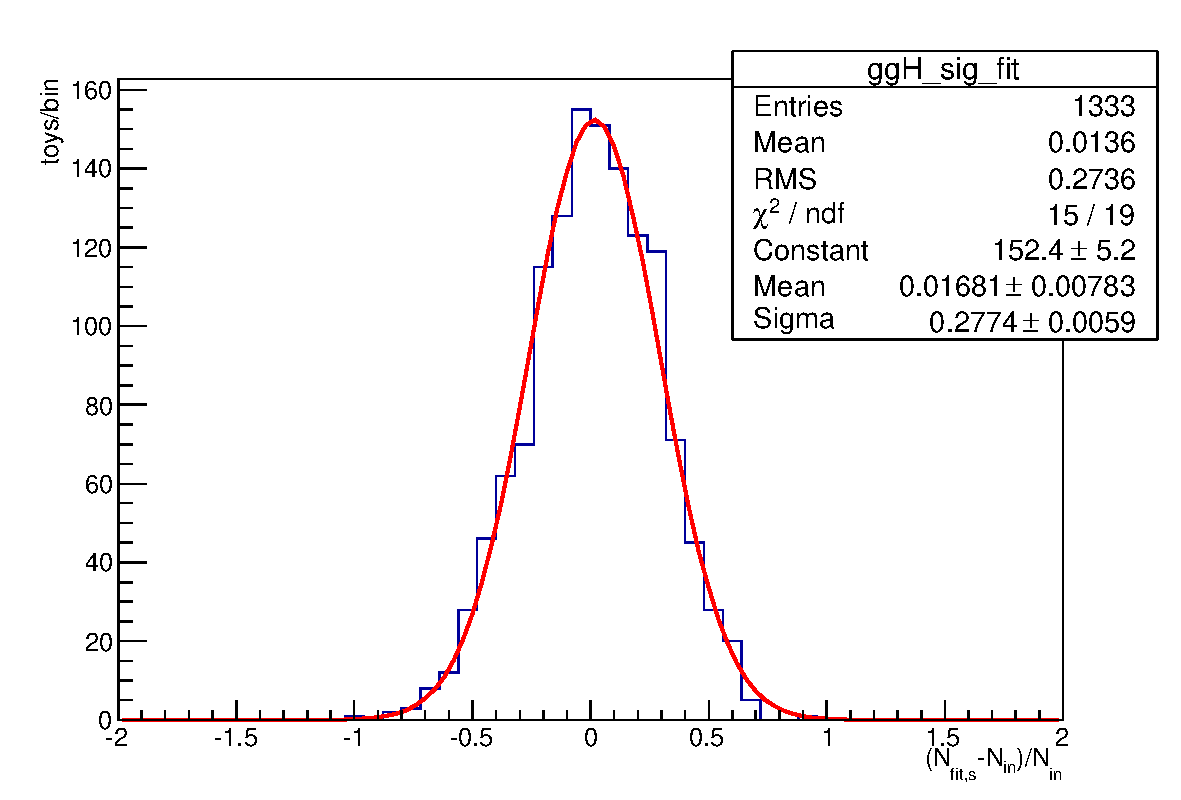
\includegraphics[width=.45\textwidth]{figures/norm_inj125_0j_125_sfit_ggH_hww_statonly.pdf}
}
\subfigure[qqWW]{
\centering
\label{subfig:qqww}
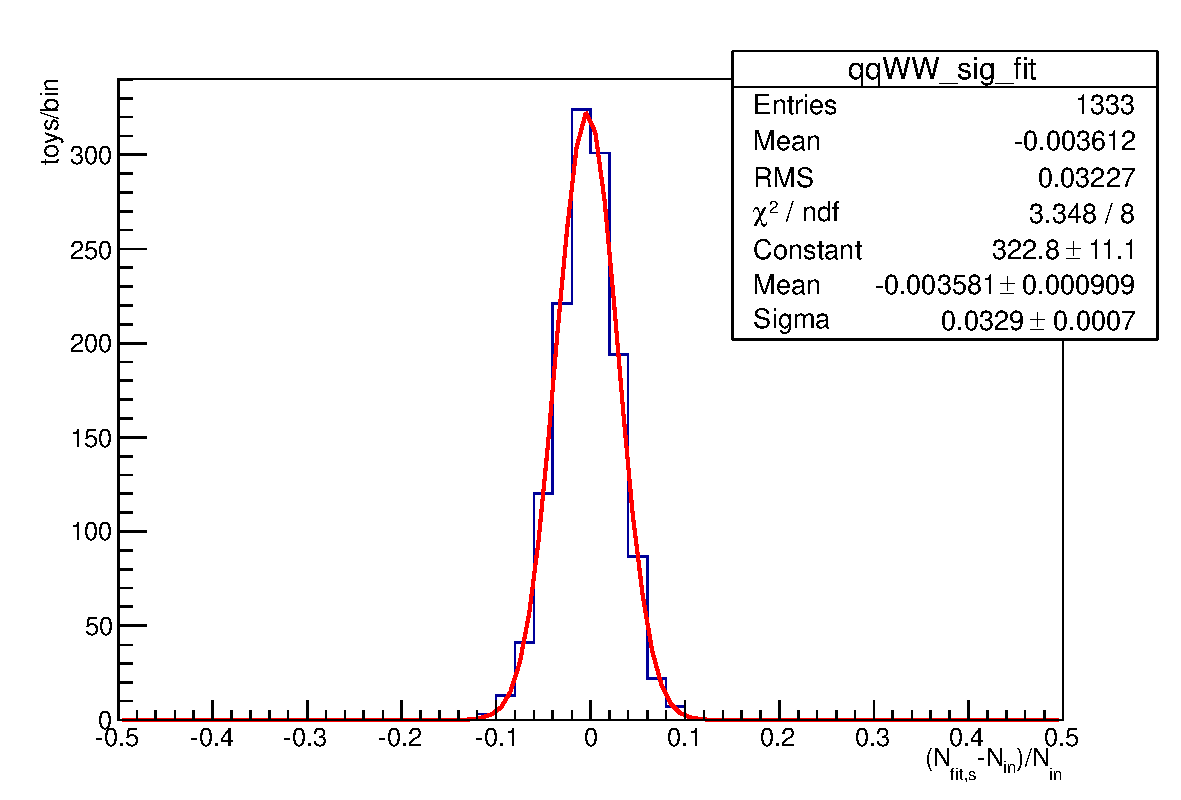
\includegraphics[width=.45\textwidth]{figures/norm_inj125_0j_125_sfit_qqWW_hww_statonly.pdf}
}\\
\subfigure[ggWW]{
\centering
\label{subfig:ggww}
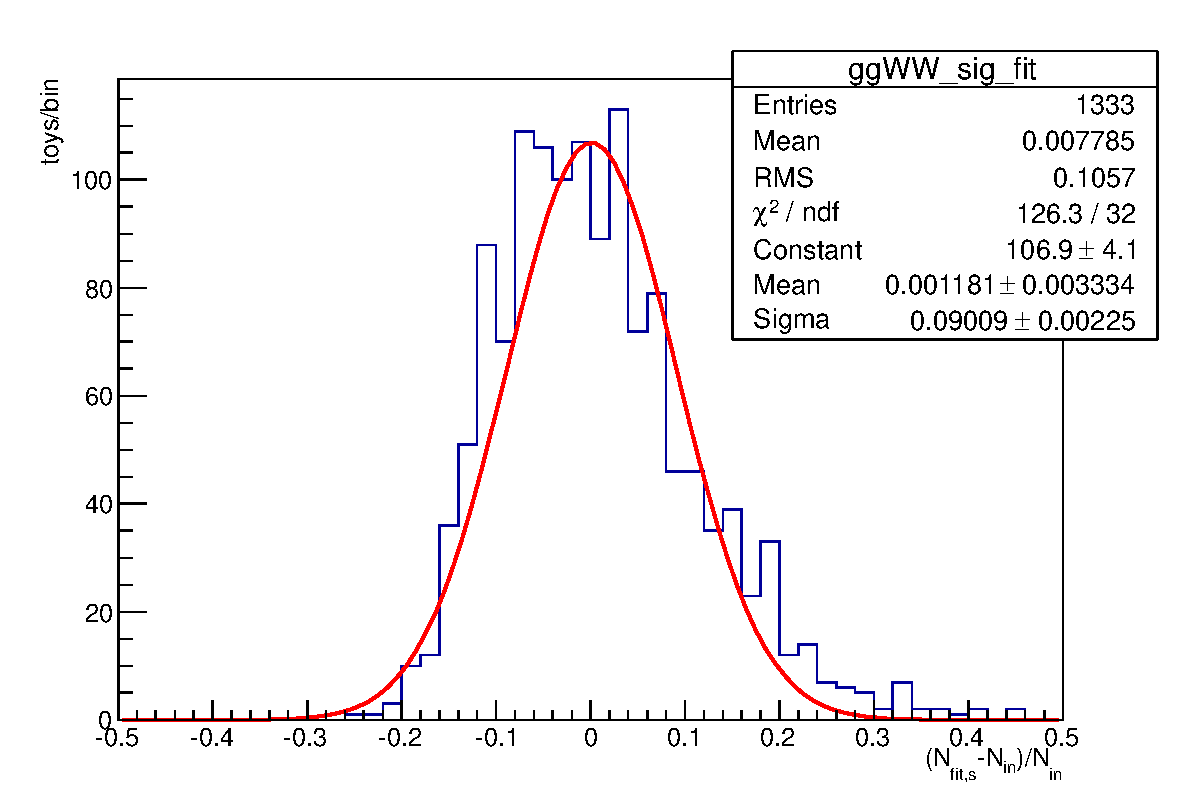
\includegraphics[width=.45\textwidth]{figures/norm_inj125_0j_125_sfit_ggWW_hww_statonly.pdf}
} 
\subfigure[Top]{
\centering
\label{subfig:top}
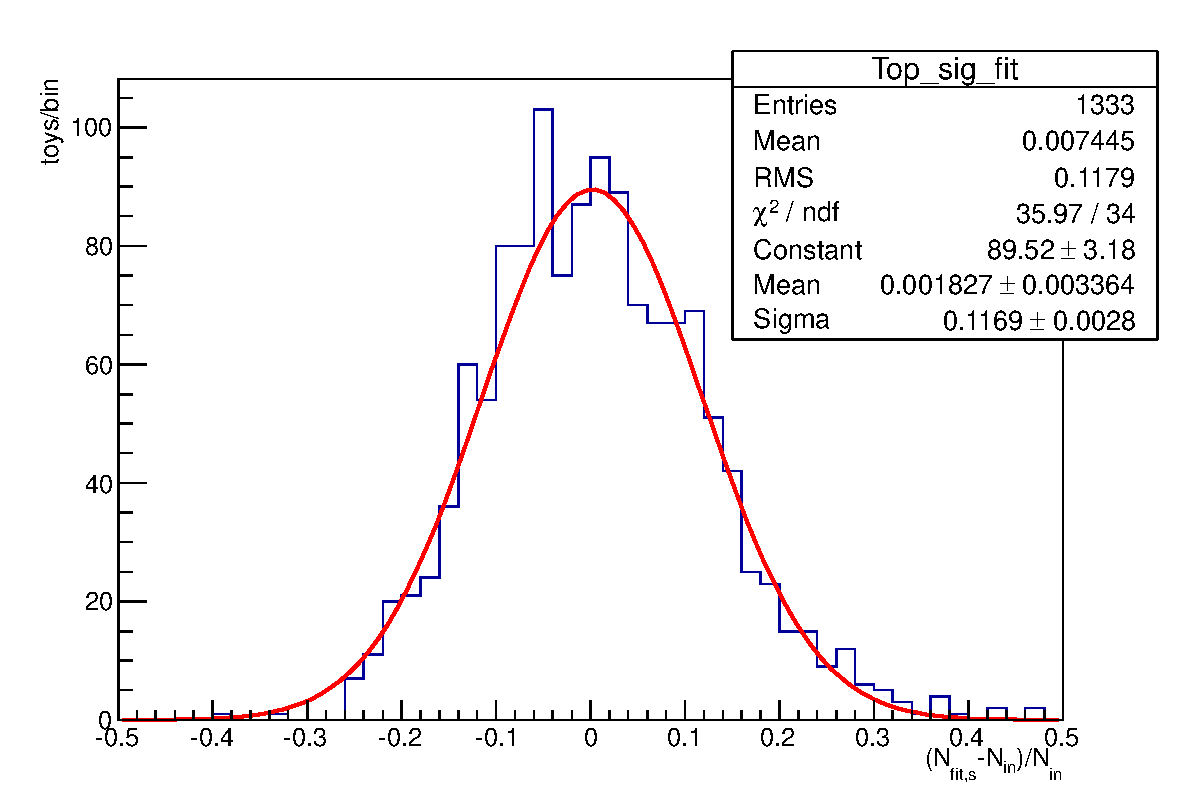
\includegraphics[width=.45\textwidth]{figures/norm_inj125_0j_125_sfit_Top_hww_statonly.pdf}
} \\
\subfigure[WjetsE]{
\centering
\label{subfig:wjetse}
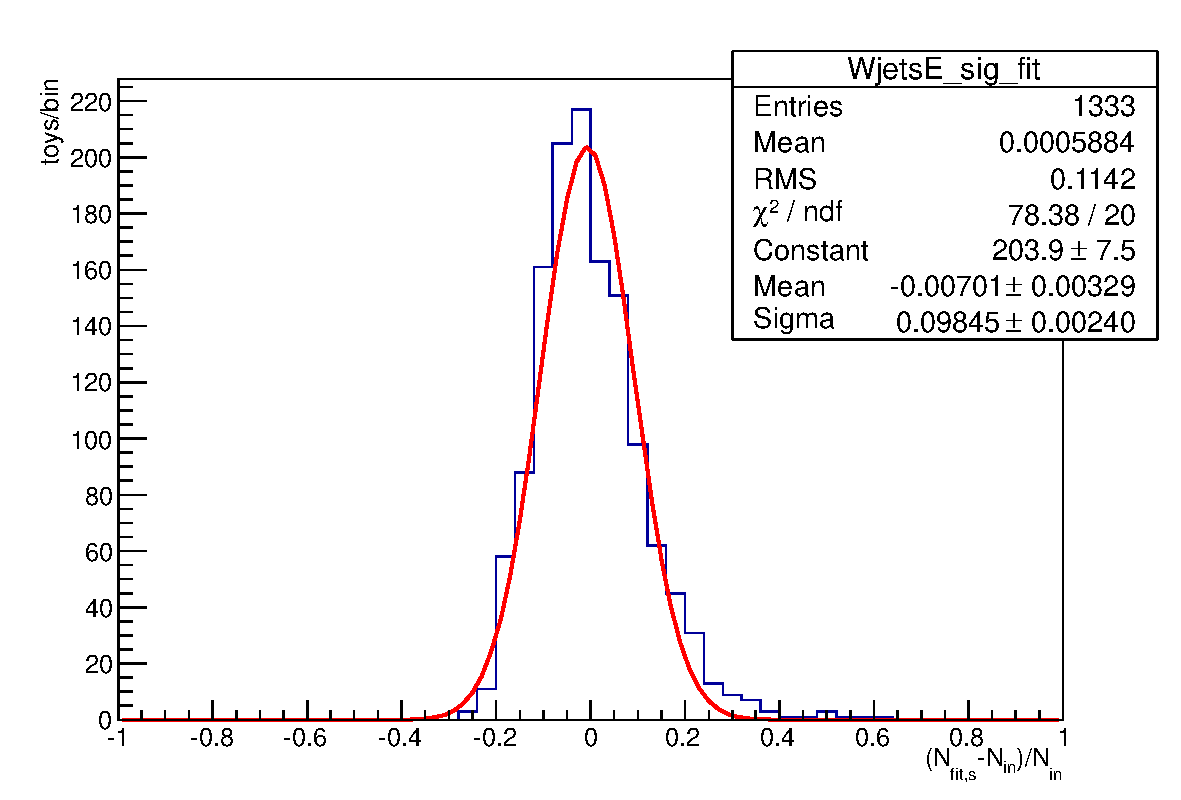
\includegraphics[width=.45\textwidth]{figures/norm_inj125_0j_125_sfit_WjetsE_hww_statonly.pdf}
} 
\subfigure[WjetsM]{
\centering
\label{subfig:wjetsm}
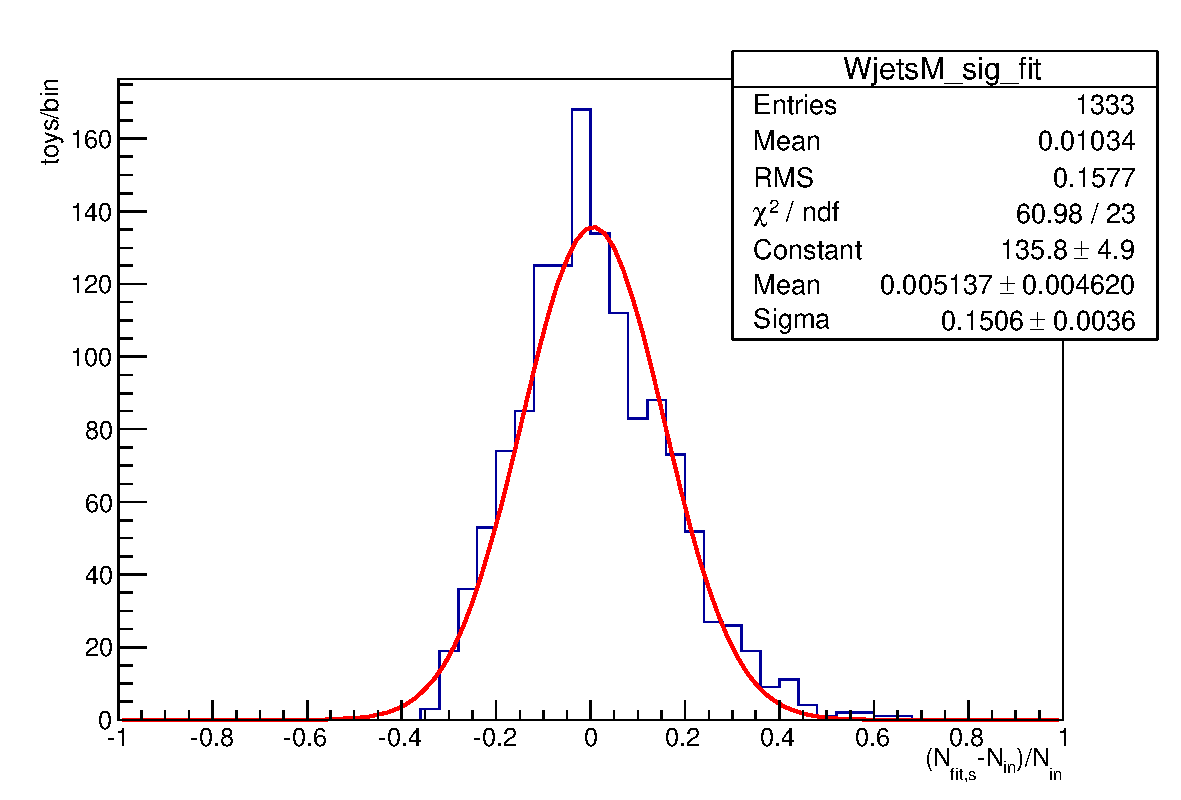
\includegraphics[width=.45\textwidth]{figures/norm_inj125_0j_125_sfit_WjetsM_hww_statonly.pdf}
} 
\subfigure[W$\gamma$]{
\centering
\label{subfig:wgamma}
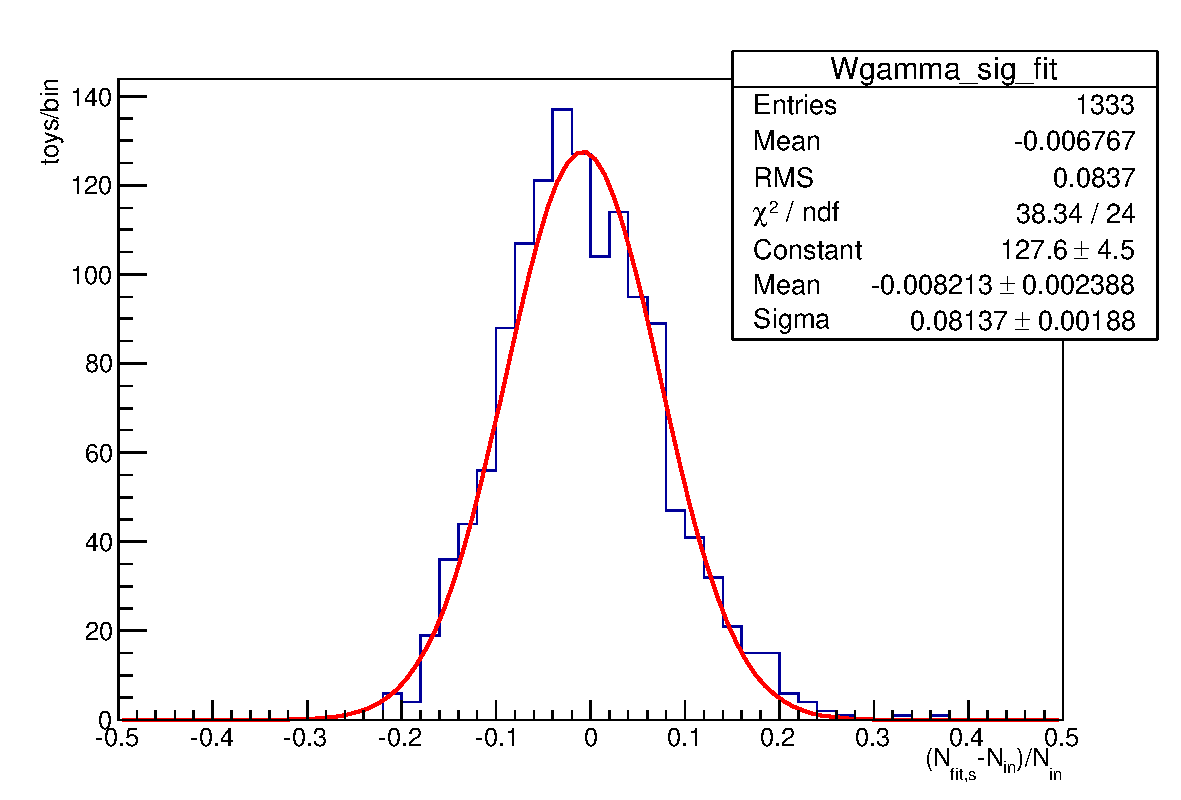
\includegraphics[width=.45\textwidth]{figures/norm_inj125_0j_125_sfit_Wgamma_hww_statonly.pdf}
} 
\subfigure[W$\gamma^*$]{
\centering
\label{subfig:wg3l}
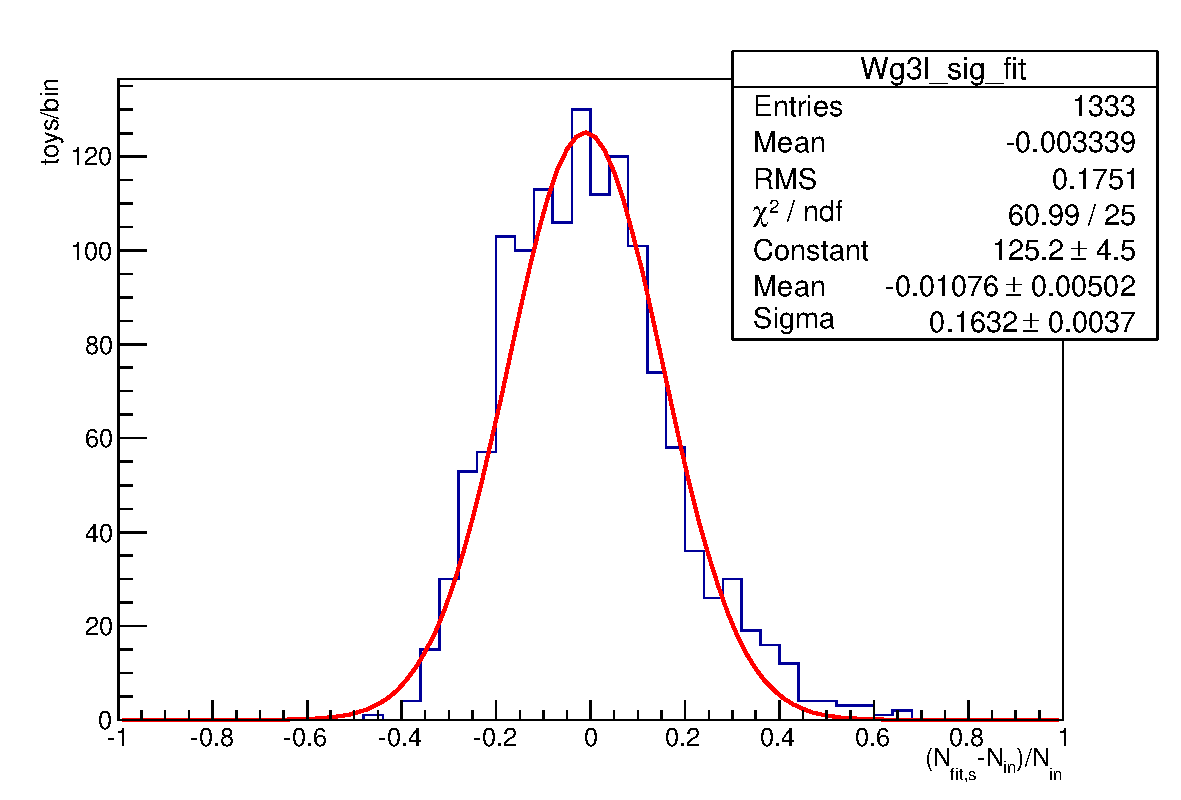
\includegraphics[width=.45\textwidth]{figures/norm_inj125_0j_125_sfit_Wg3l_hww_statonly.pdf}
} 

\caption{The relative fit bias $(N_{\text fit} - N_{\text in})/N_{\text in}$ distributions 
of the main signal and background processes in the toy MC based fit studies in the {\bf 0-Jet bin}. 
The toy datasets are generated sampling {\bf only statistics of the templates}. }
\label{fig:toyfit_statonly_0j}
\end{figure}
%%%%%%%%%%%%%%%%%%%%%%%%%%%%%%%%%%%%


%%%%%%%%%%%%%%%%%%%%%%%%%%%%%%%%%%%%
\begin{figure}[!hbtp]
\centering
\subfigure[ggH]{
\centering
\label{subfig:ggh}
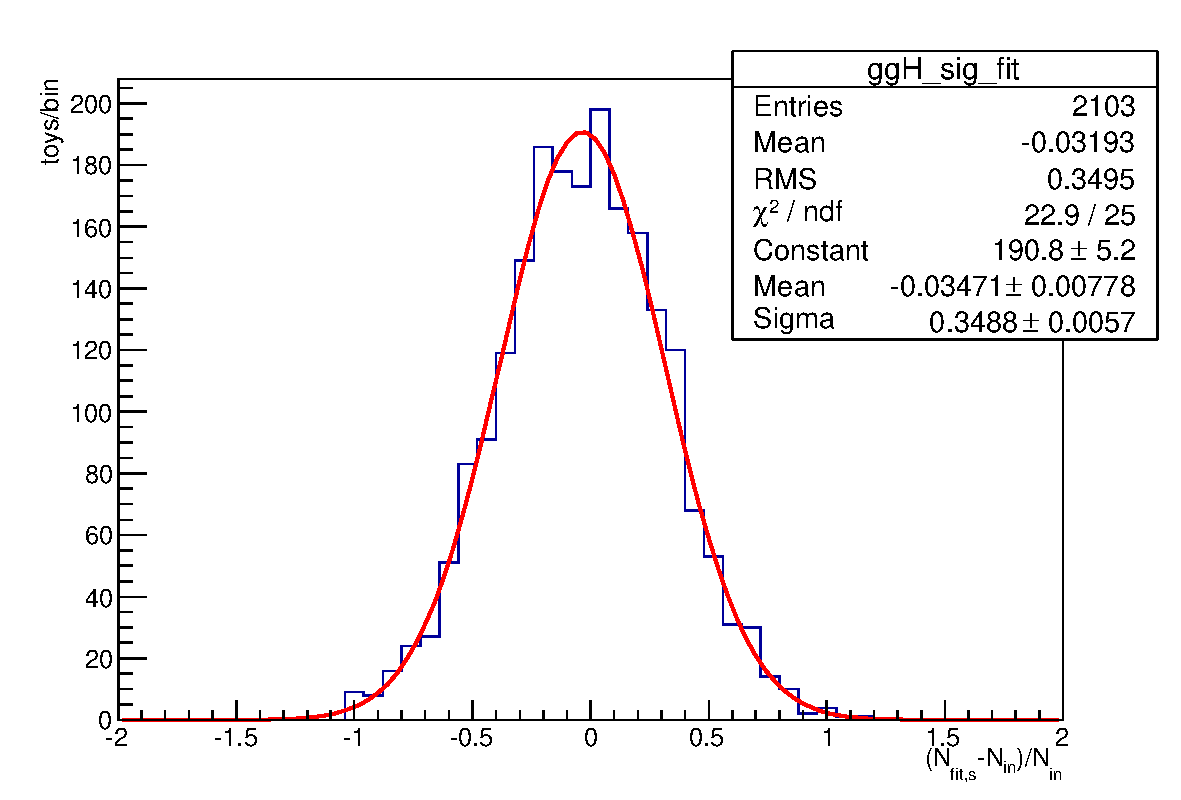
\includegraphics[width=.45\textwidth]{figures/norm_inj125_1j_125_sfit_ggH_hww_statonly.pdf}
}
\subfigure[qqWW]{
\centering
\label{subfig:qqww}
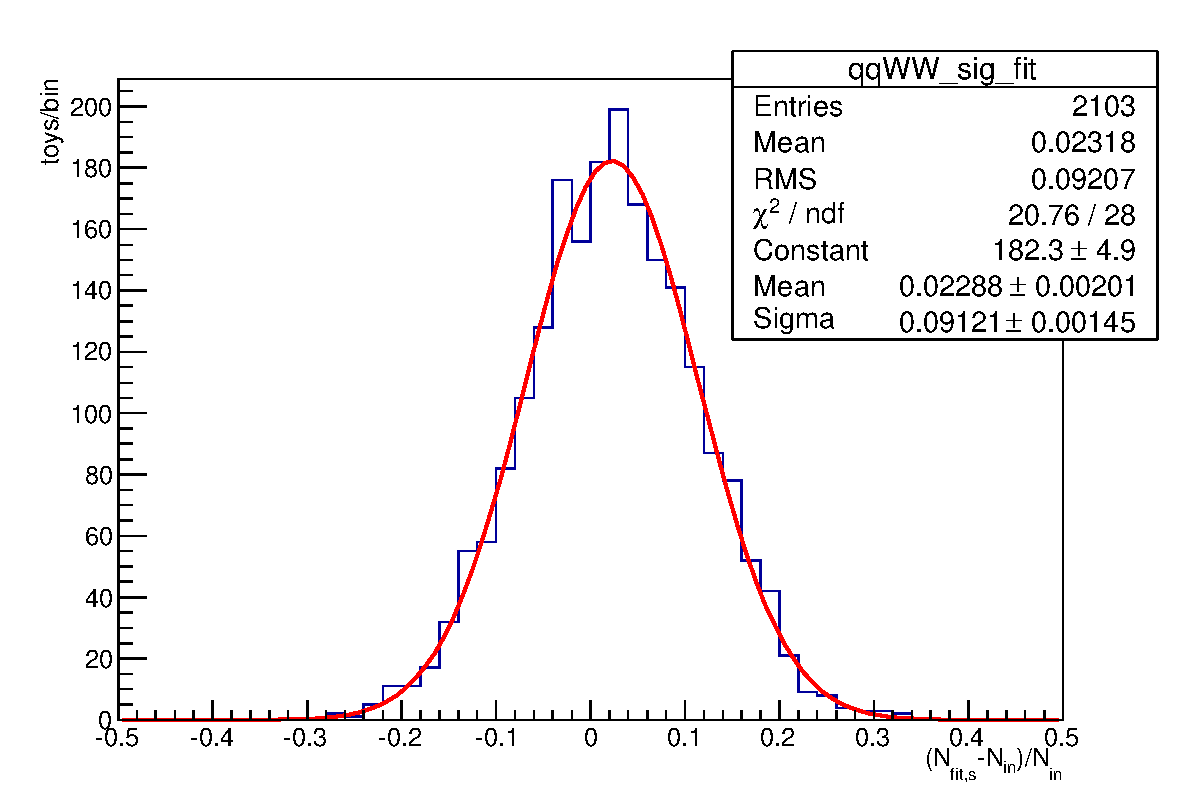
\includegraphics[width=.45\textwidth]{figures/norm_inj125_1j_125_sfit_qqWW_hww_statonly.pdf}
}\\
\subfigure[ggWW]{
\centering
\label{subfig:ggww}
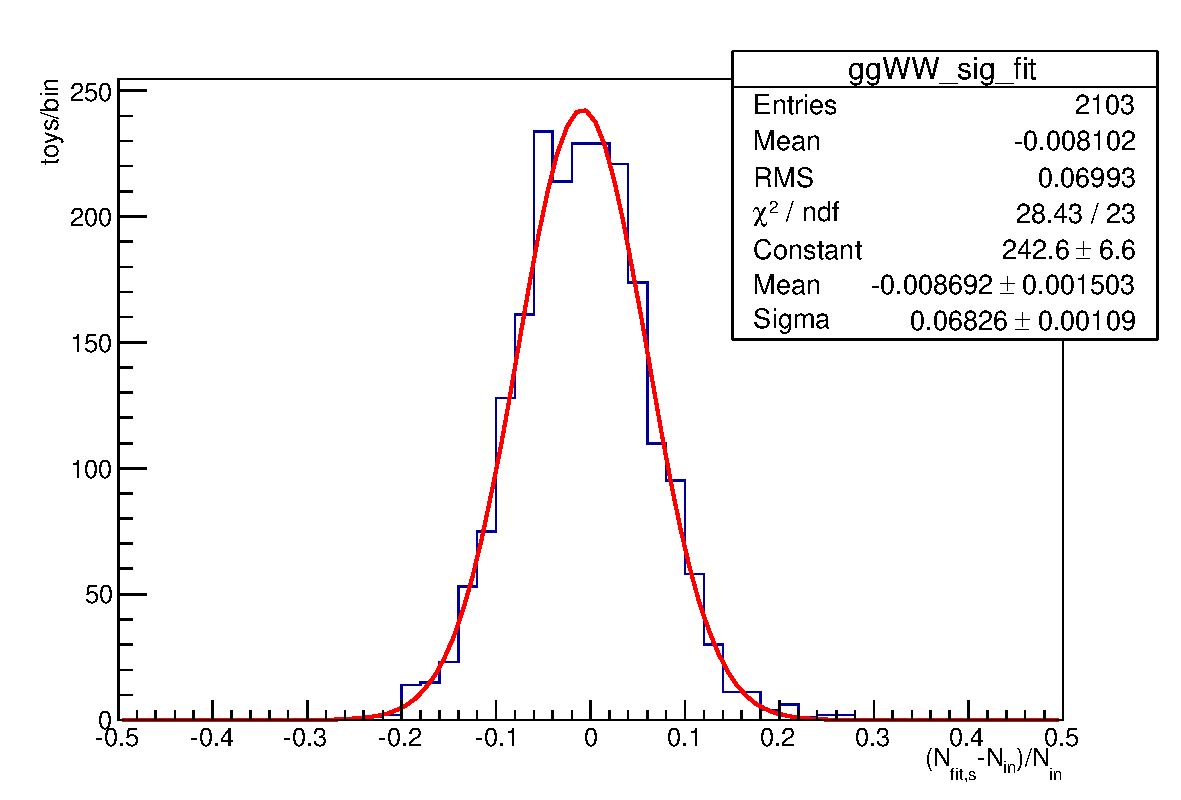
\includegraphics[width=.45\textwidth]{figures/norm_inj125_1j_125_sfit_ggWW_hww_statonly.pdf}
} 
\subfigure[Top]{
\centering
\label{subfig:top}
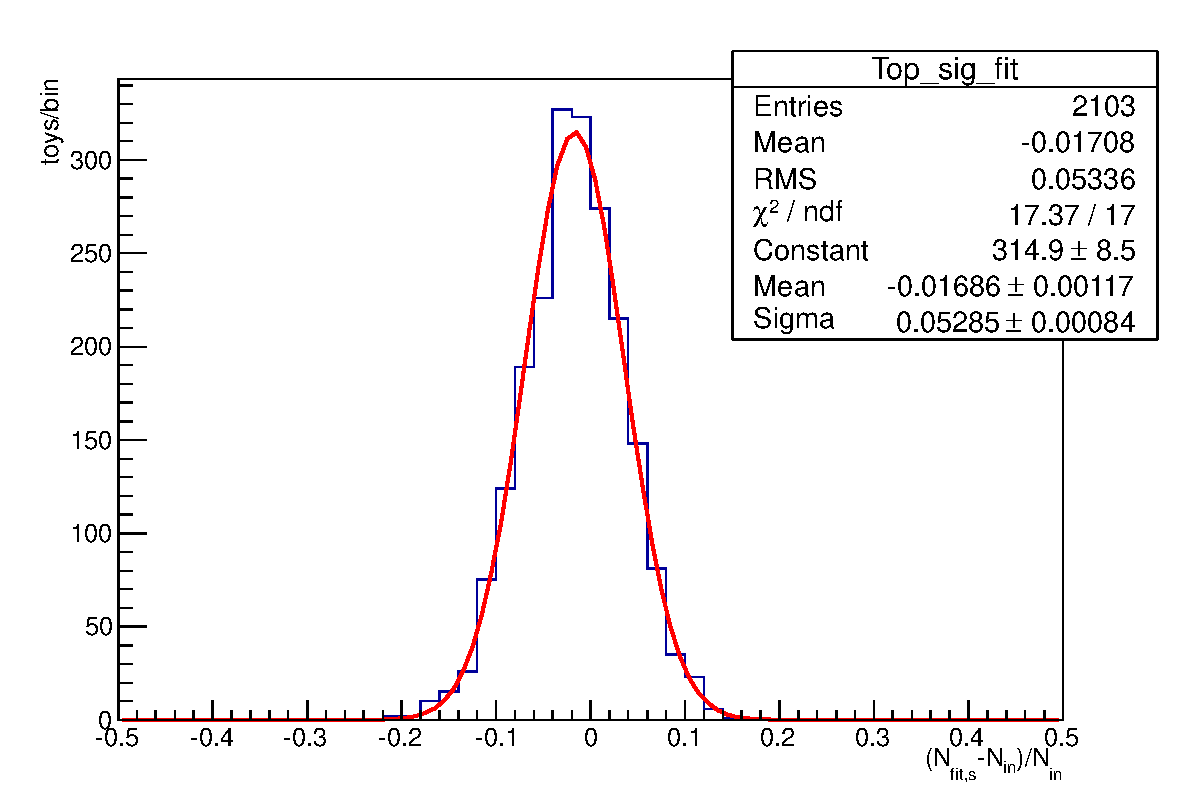
\includegraphics[width=.45\textwidth]{figures/norm_inj125_1j_125_sfit_Top_hww_statonly.pdf}
} \\
\subfigure[WjetsE]{
\centering
\label{subfig:wjetse}
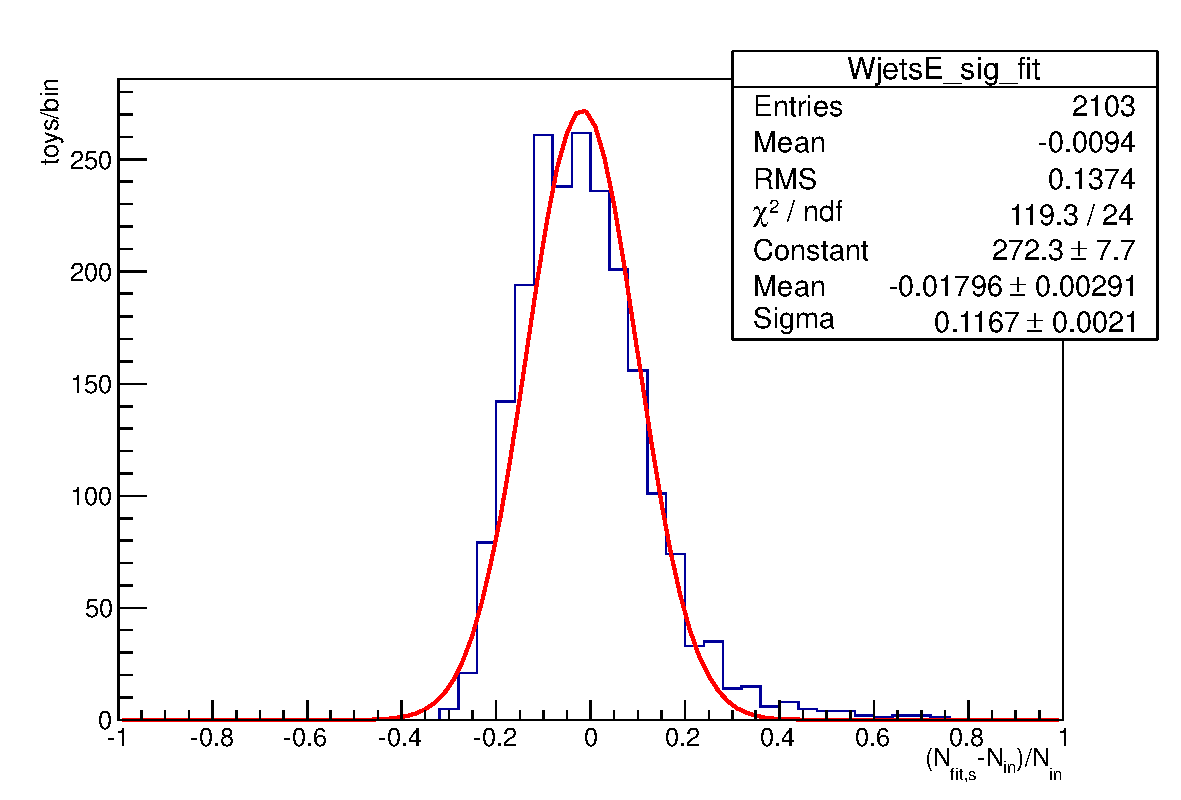
\includegraphics[width=.45\textwidth]{figures/norm_inj125_1j_125_sfit_WjetsE_hww_statonly.pdf}
} 
\subfigure[WjetsM]{
\centering
\label{subfig:wjetsm}
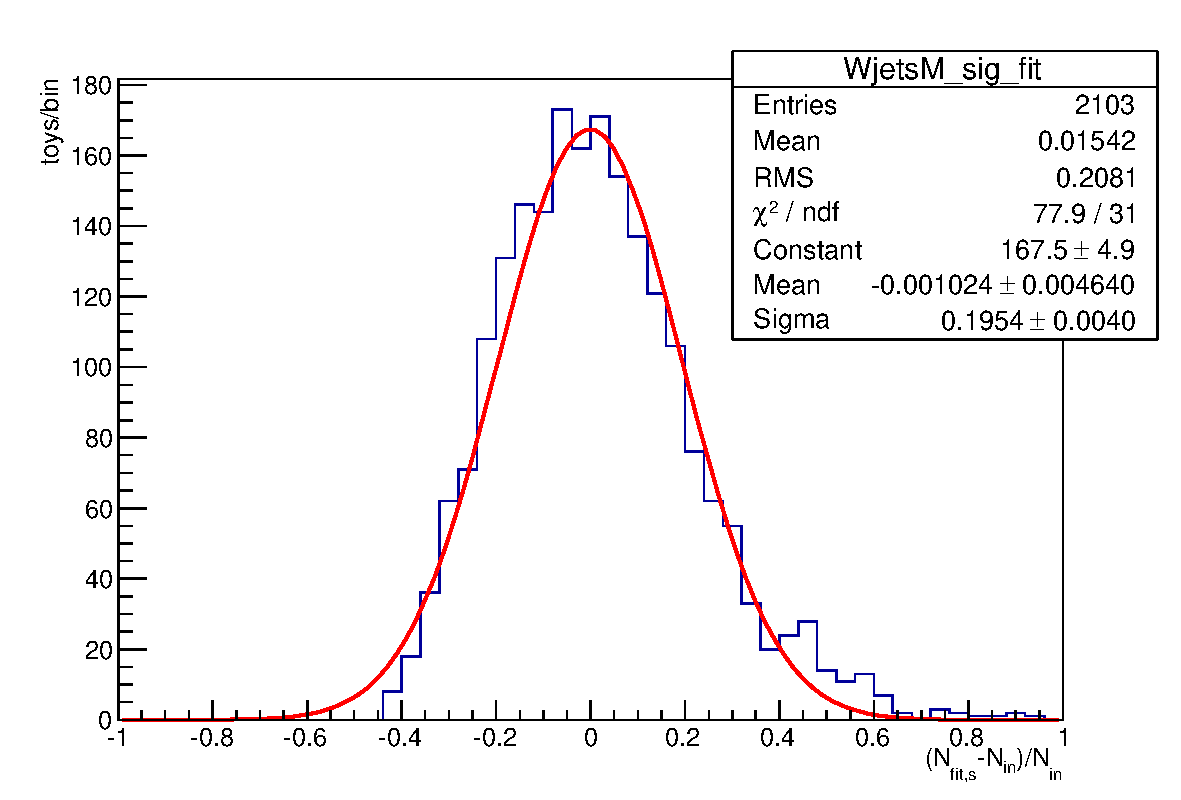
\includegraphics[width=.45\textwidth]{figures/norm_inj125_1j_125_sfit_WjetsM_hww_statonly.pdf}
} 
\subfigure[W$\gamma$]{
\centering
\label{subfig:wgamma}
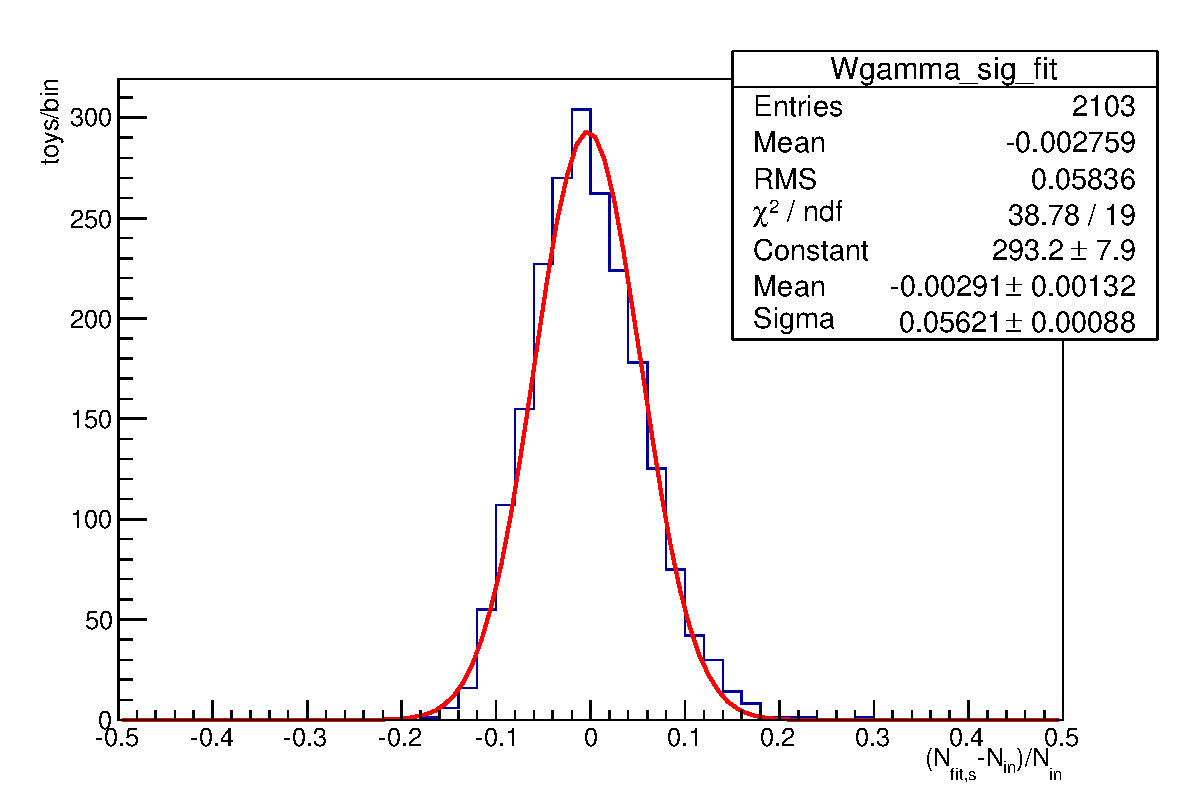
\includegraphics[width=.45\textwidth]{figures/norm_inj125_1j_125_sfit_Wgamma_hww_statonly.pdf}
} 
\subfigure[W$\gamma^*$]{
\centering
\label{subfig:wg3l}
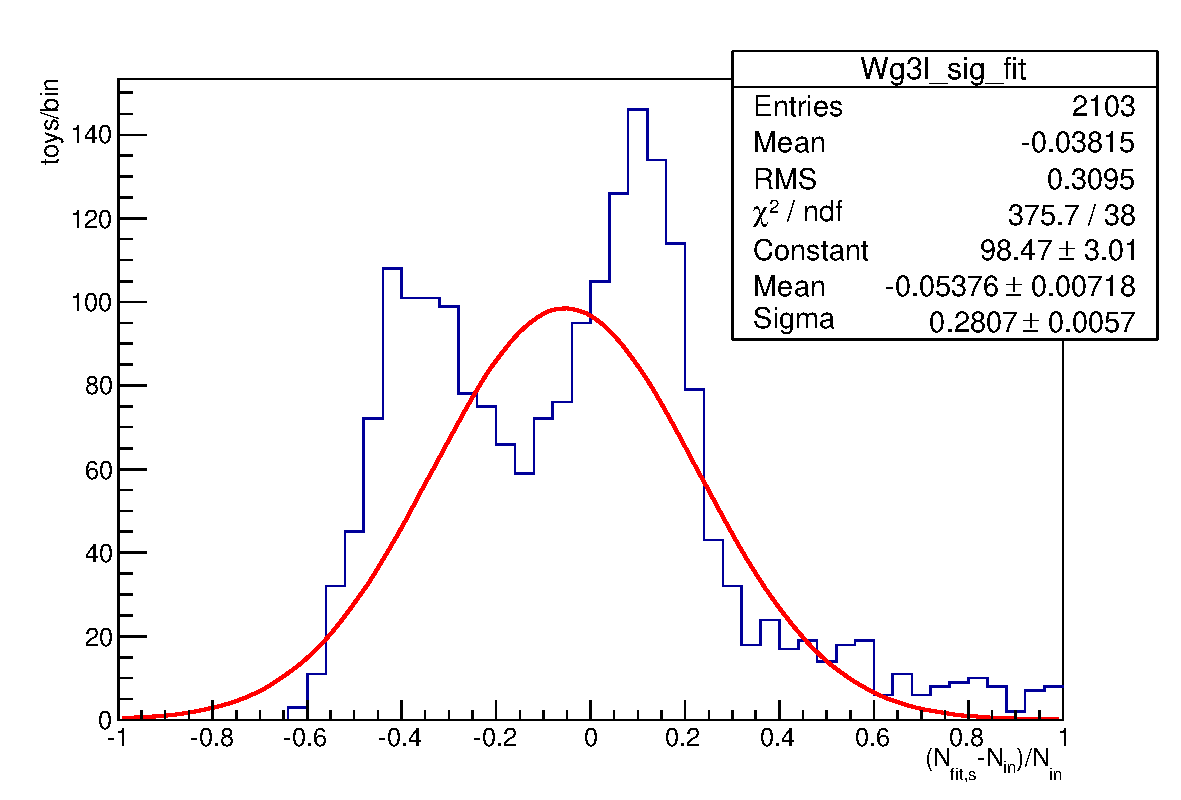
\includegraphics[width=.45\textwidth]{figures/norm_inj125_1j_125_sfit_Wg3l_hww_statonly.pdf}
} 

\caption{The relative fit bias $(N_{\text fit} - N_{\text in})/N_{\text in}$ distributions 
of the main signal and background processes in the toy MC based fit studies in the {\bf 1-Jet bin}. 
The toy datasets are generated sampling {\bf only statistics of the templates}. }
\label{fig:toyfit_statonly_1j}
\end{figure}
%% %%%%%%%%%%%%%%%%%%%%%%%%%%%%%%%%%%%%


%%%%%%%%%%%%%%%%%%%%%%%%%%%%%%%%%%%%
\begin{figure}[!hbtp]
\centering
\subfigure[ggH]{
\centering
\label{subfig:ggh}
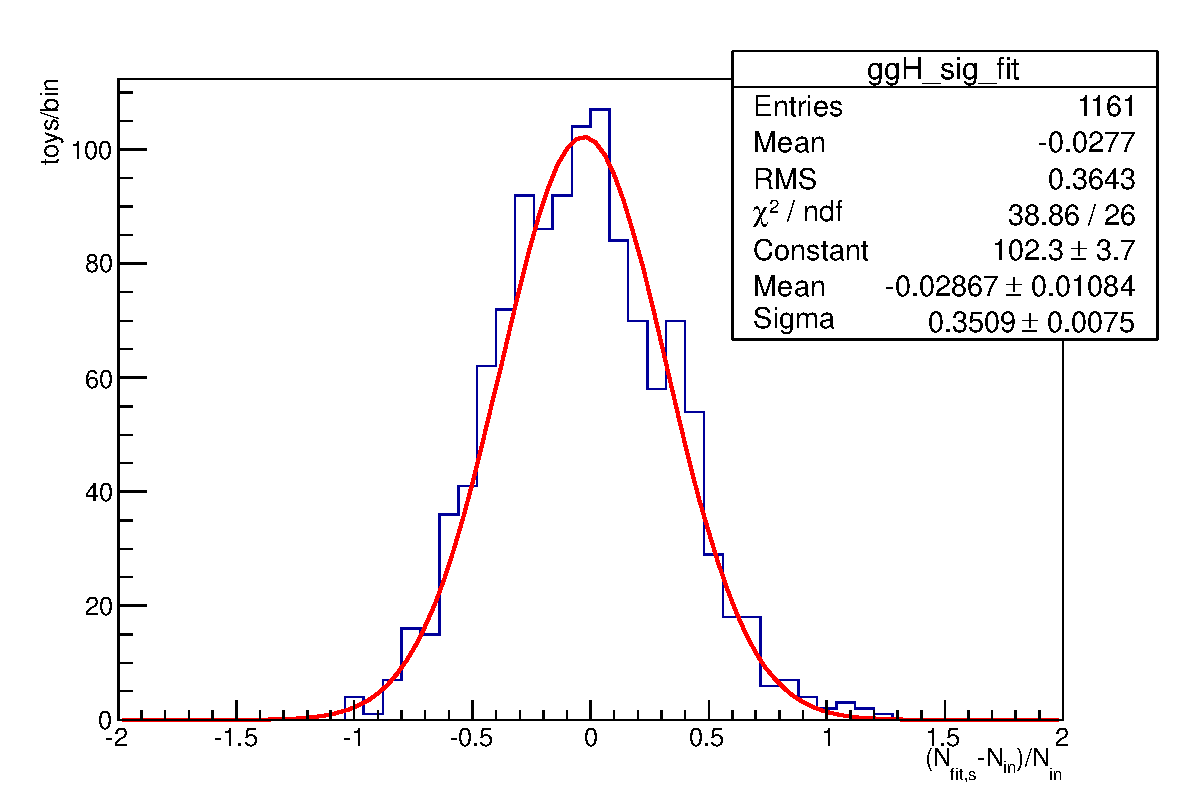
\includegraphics[width=.45\textwidth]{figures/norm_inj125_0j_125_sfit_ggH_hww.pdf}
}
\subfigure[qqWW]{
\centering
\label{subfig:qqww}
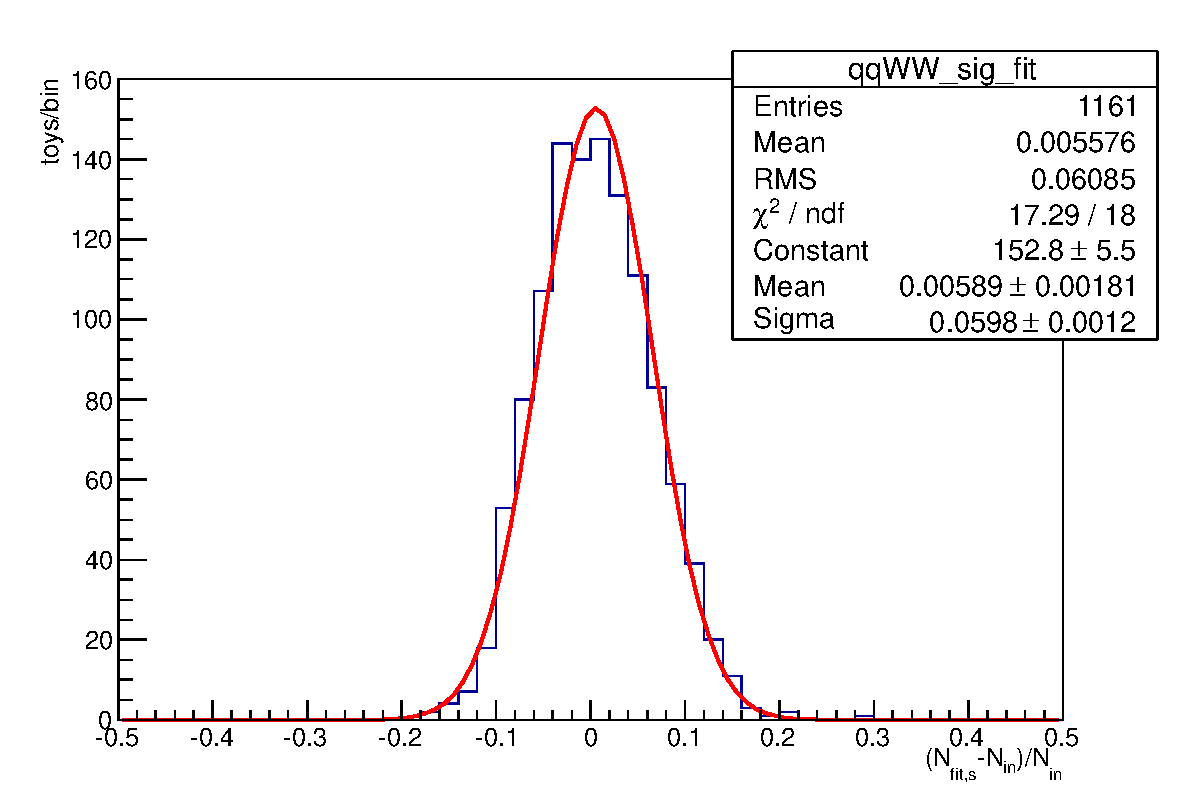
\includegraphics[width=.45\textwidth]{figures/norm_inj125_0j_125_sfit_qqWW_hww.pdf}
}\\
\subfigure[ggWW]{
\centering
\label{subfig:ggww}
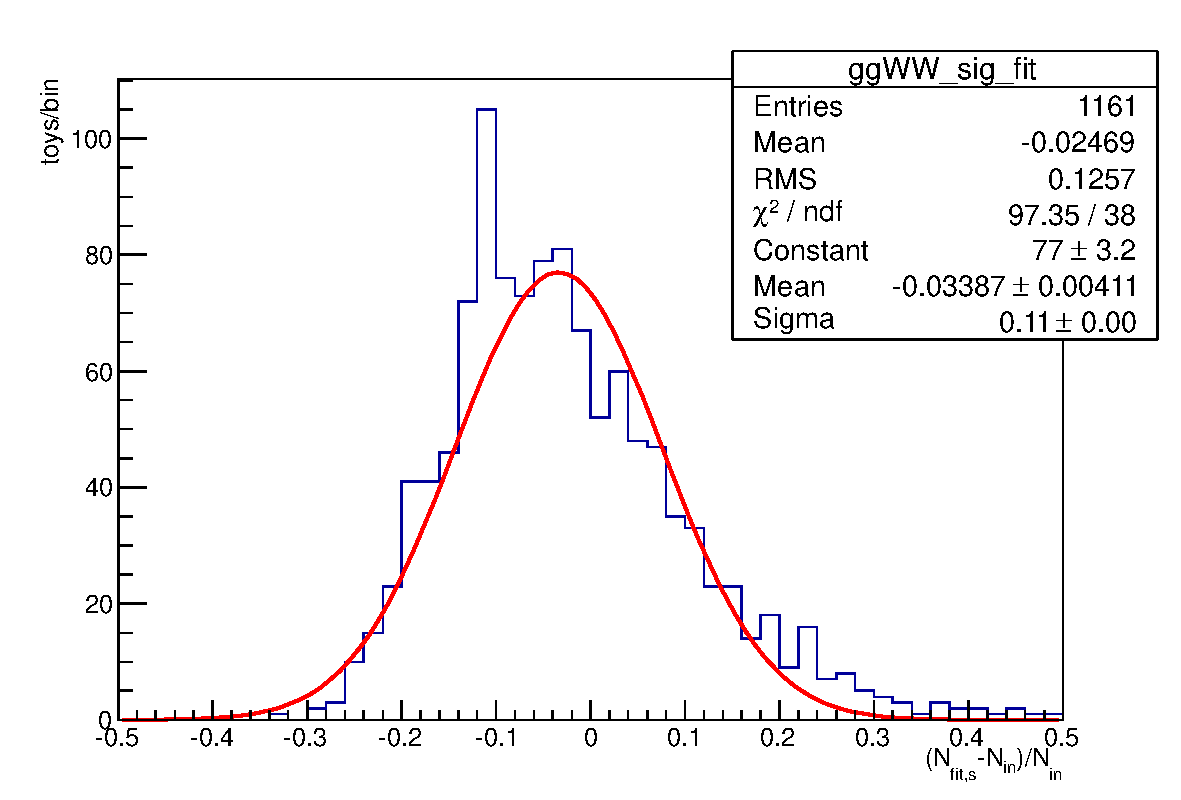
\includegraphics[width=.45\textwidth]{figures/norm_inj125_0j_125_sfit_ggWW_hww.pdf}
} 
\subfigure[Top]{
\centering
\label{subfig:top}
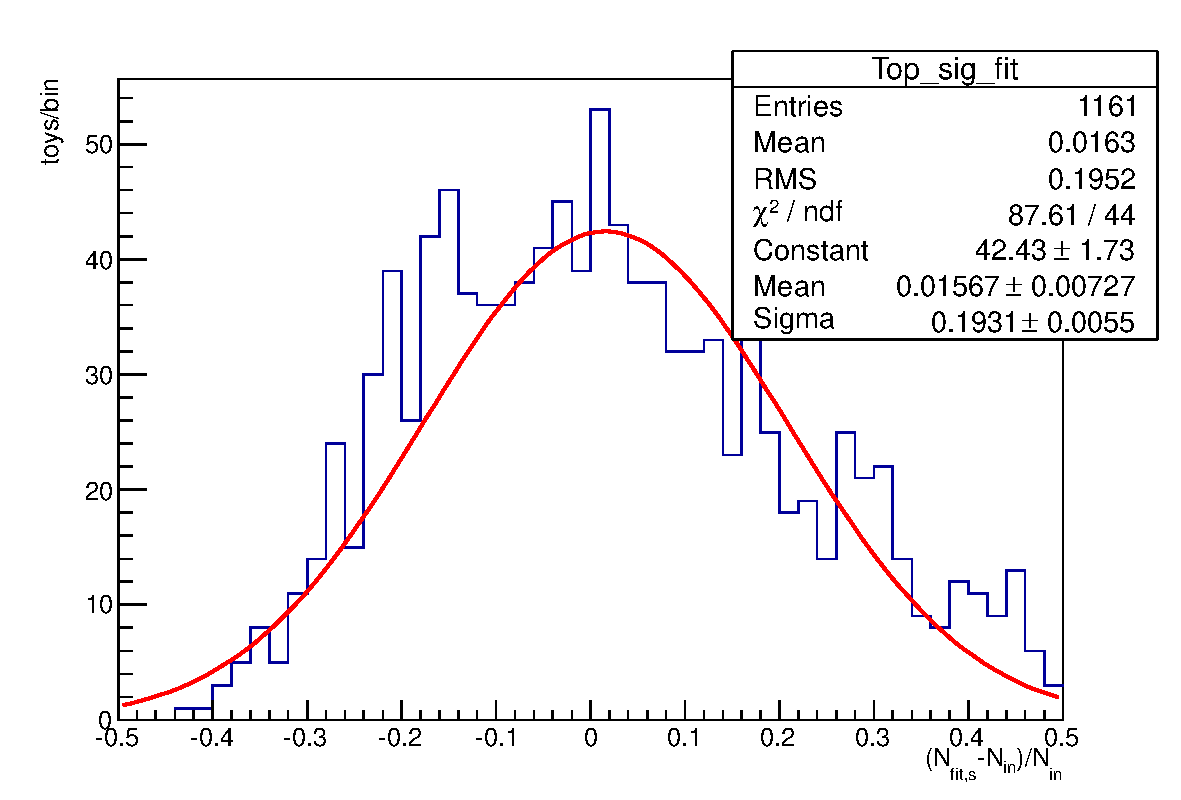
\includegraphics[width=.45\textwidth]{figures/norm_inj125_0j_125_sfit_Top_hww.pdf}
} \\
\subfigure[WjetsE]{
\centering
\label{subfig:wjetse}
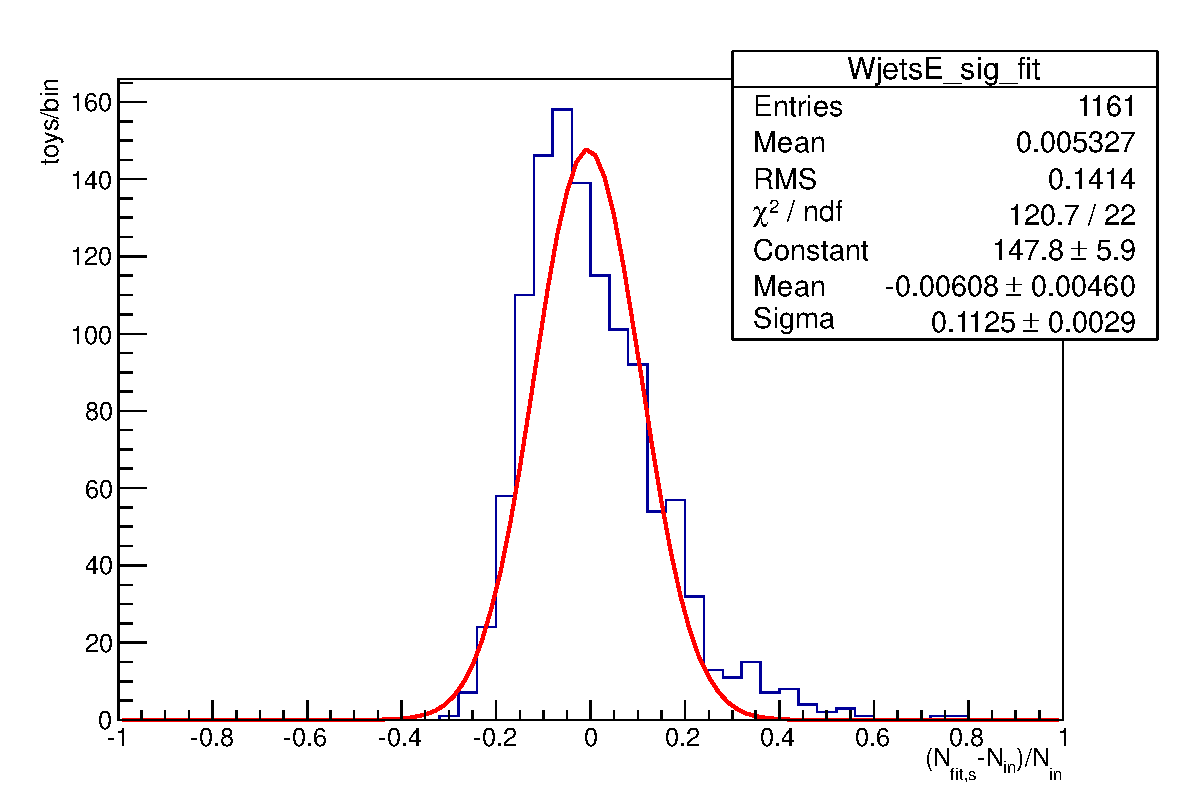
\includegraphics[width=.45\textwidth]{figures/norm_inj125_0j_125_sfit_WjetsE_hww.pdf}
} 
\subfigure[WjetsM]{
\centering
\label{subfig:wjetsm}
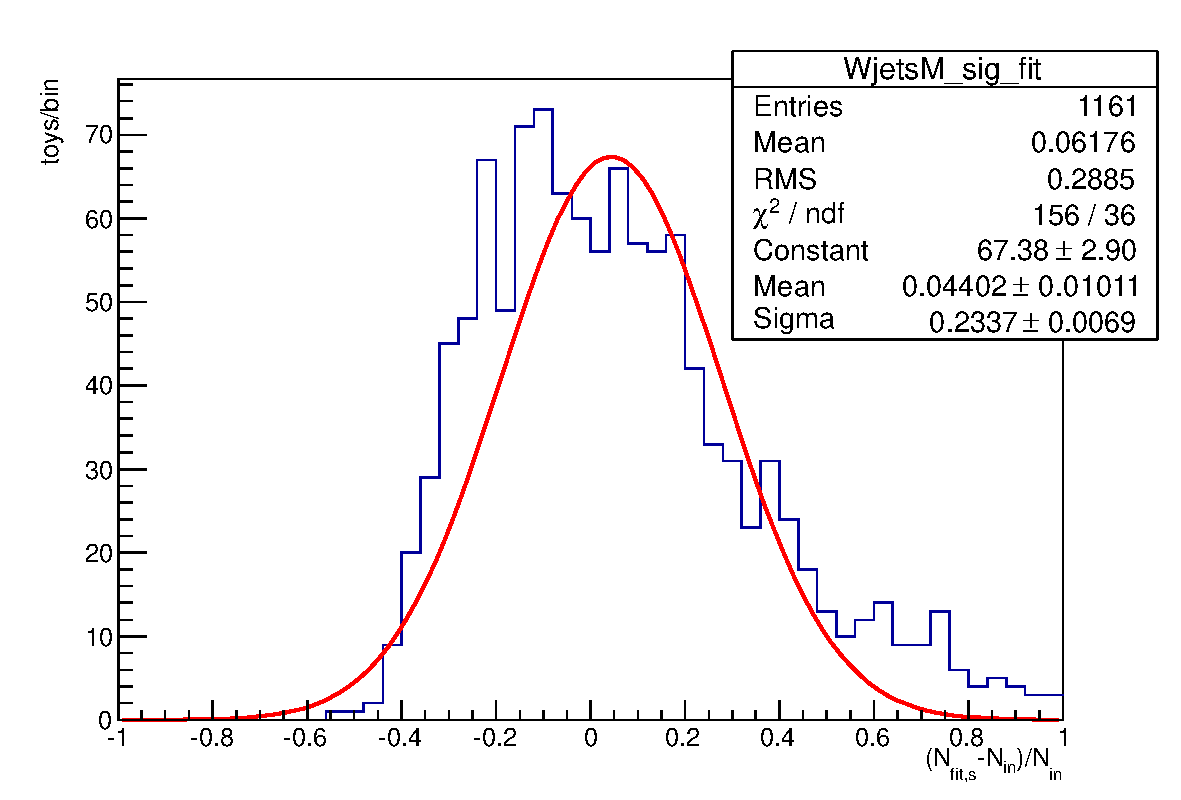
\includegraphics[width=.45\textwidth]{figures/norm_inj125_0j_125_sfit_WjetsM_hww.pdf}
} 
\subfigure[W$\gamma$]{
\centering
\label{subfig:wgamma}
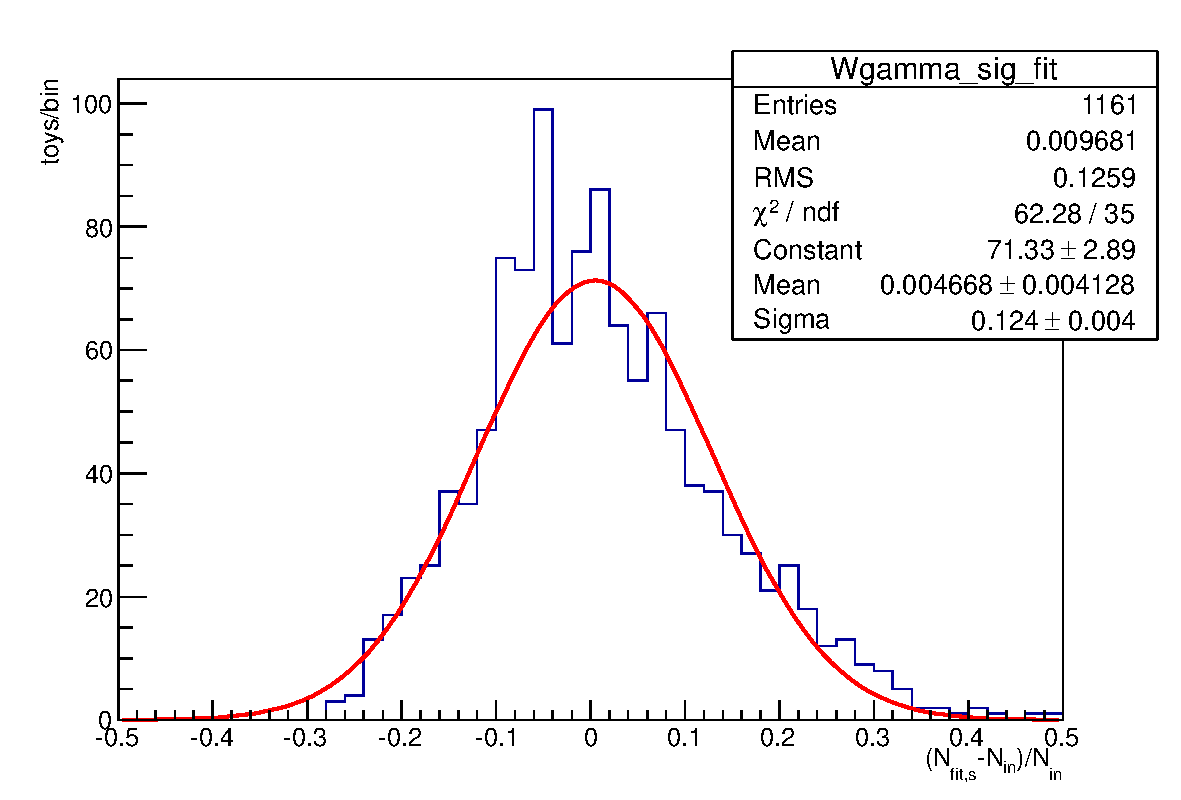
\includegraphics[width=.45\textwidth]{figures/norm_inj125_0j_125_sfit_Wgamma_hww.pdf}
} 
\subfigure[W$\gamma^*$]{
\centering
\label{subfig:wg3l}
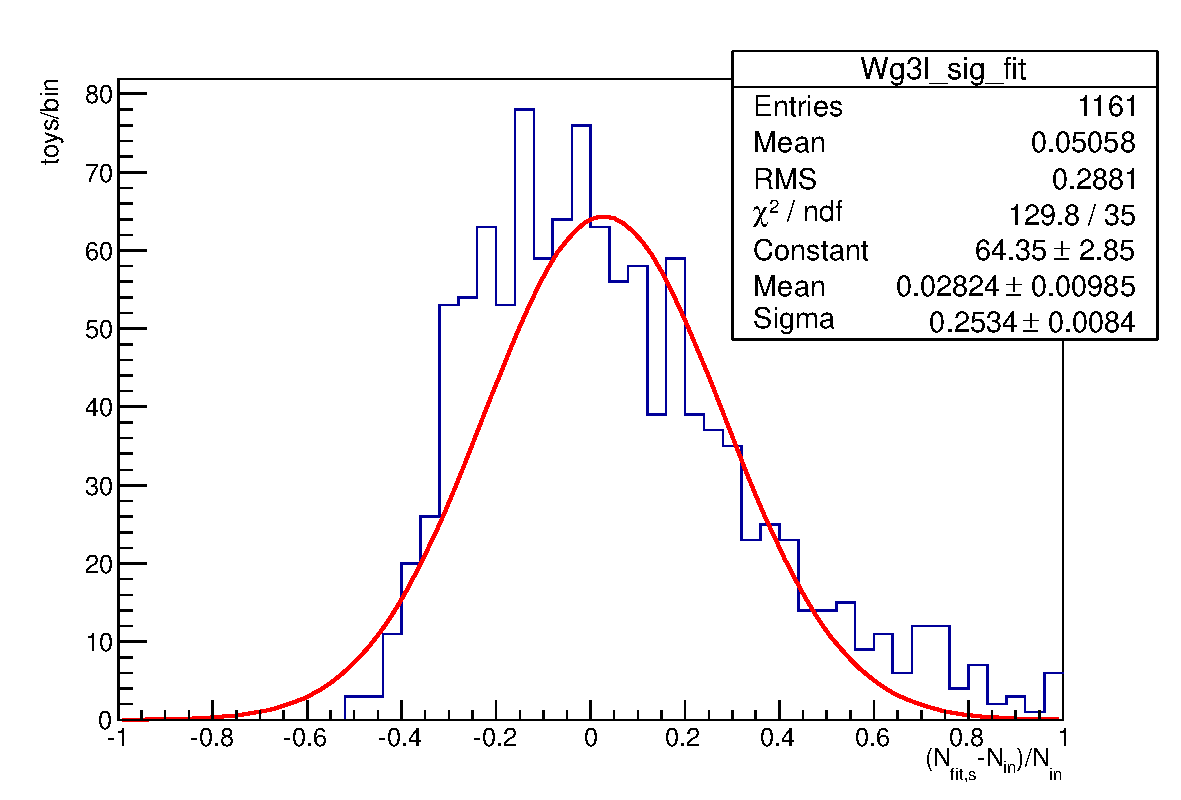
\includegraphics[width=.45\textwidth]{figures/norm_inj125_0j_125_sfit_Wg3l_hww.pdf}
} 

\caption{The relative fit bias $(N_{\text fit} - N_{\text in})/N_{\text in}$ distributions 
of the main signal and background processes in the toy MC based fit studies in the {\bf 0-Jet bin}. 
The toy datasets are generated sampling {\bf both statistics of the templates and systematic nusiances}. }
\label{fig:toyfit_0j}
\end{figure}
%%%%%%%%%%%%%%%%%%%%%%%%%%%%%%%%%%%%


%%%%%%%%%%%%%%%%%%%%%%%%%%%%%%%%%%%%
\begin{figure}[!hbtp]
\centering
\subfigure[ggH]{
\centering
\label{subfig:ggh}
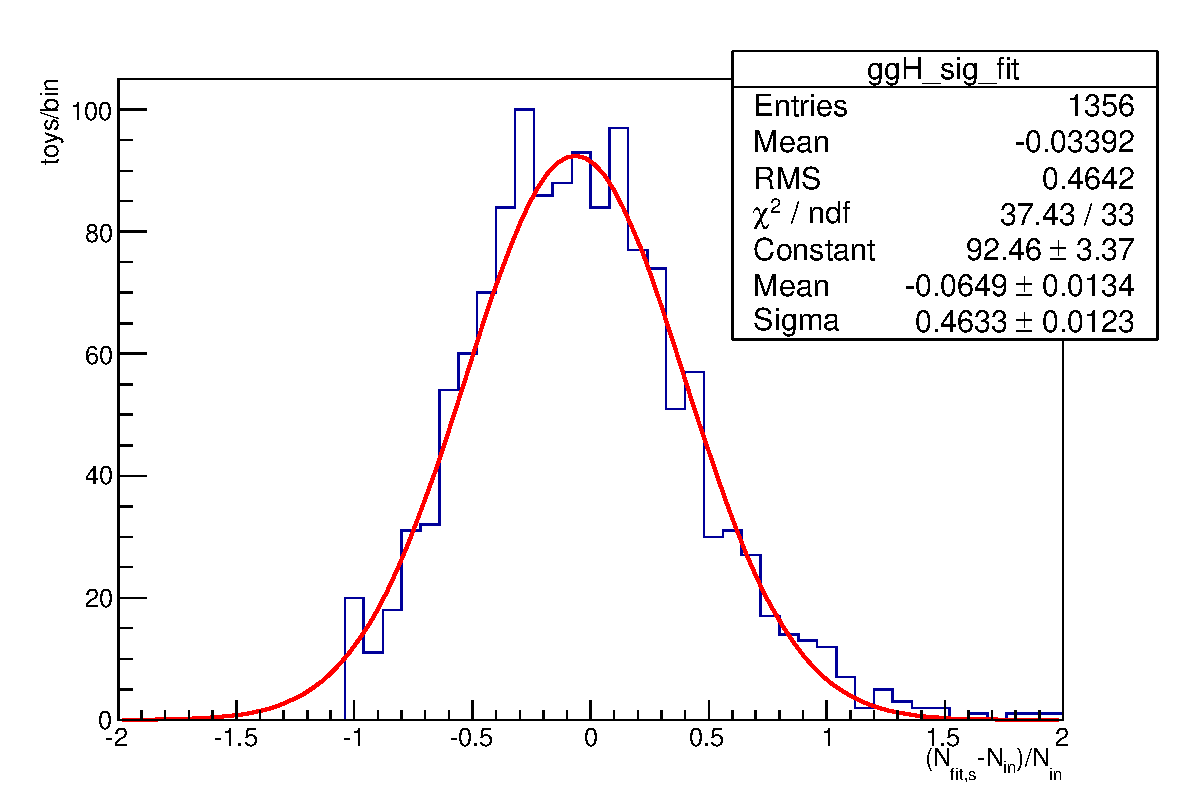
\includegraphics[width=.45\textwidth]{figures/norm_inj125_1j_125_sfit_ggH_hww.pdf}
}
\subfigure[qqWW]{
\centering
\label{subfig:qqww}
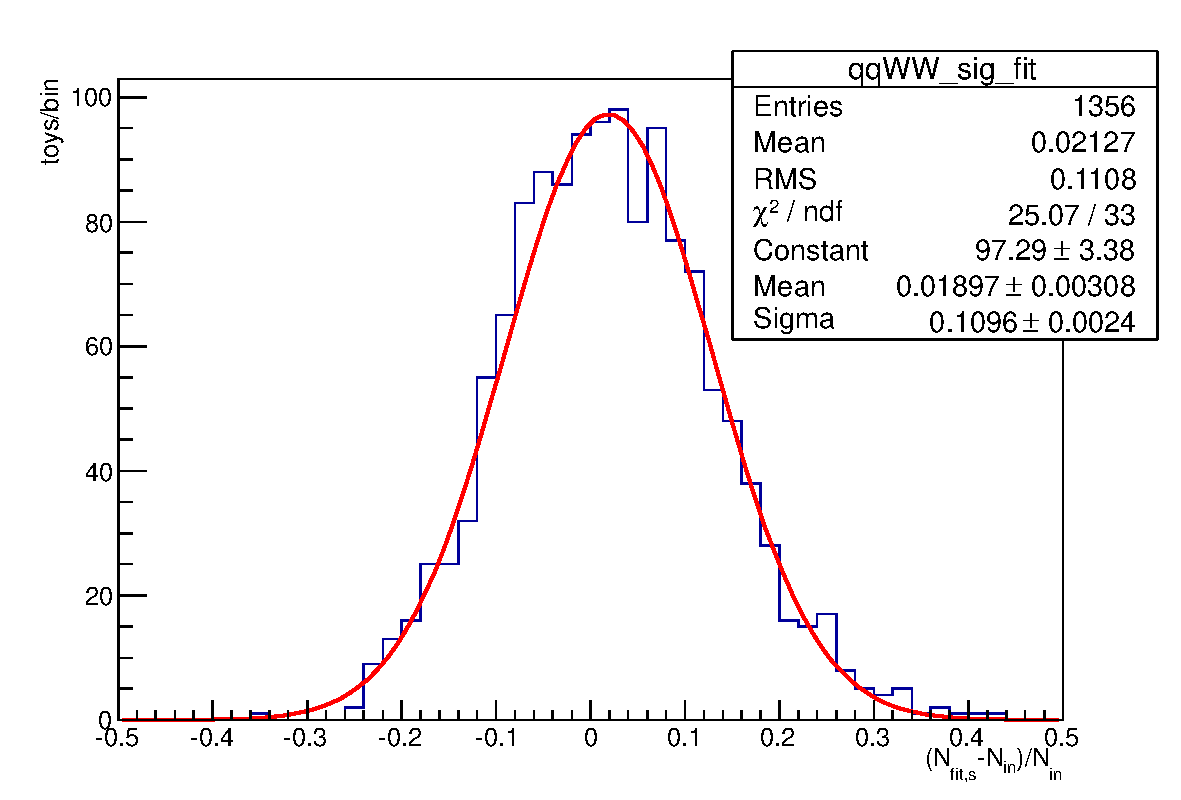
\includegraphics[width=.45\textwidth]{figures/norm_inj125_1j_125_sfit_qqWW_hww.pdf}
}\\
\subfigure[ggWW]{
\centering
\label{subfig:ggww}
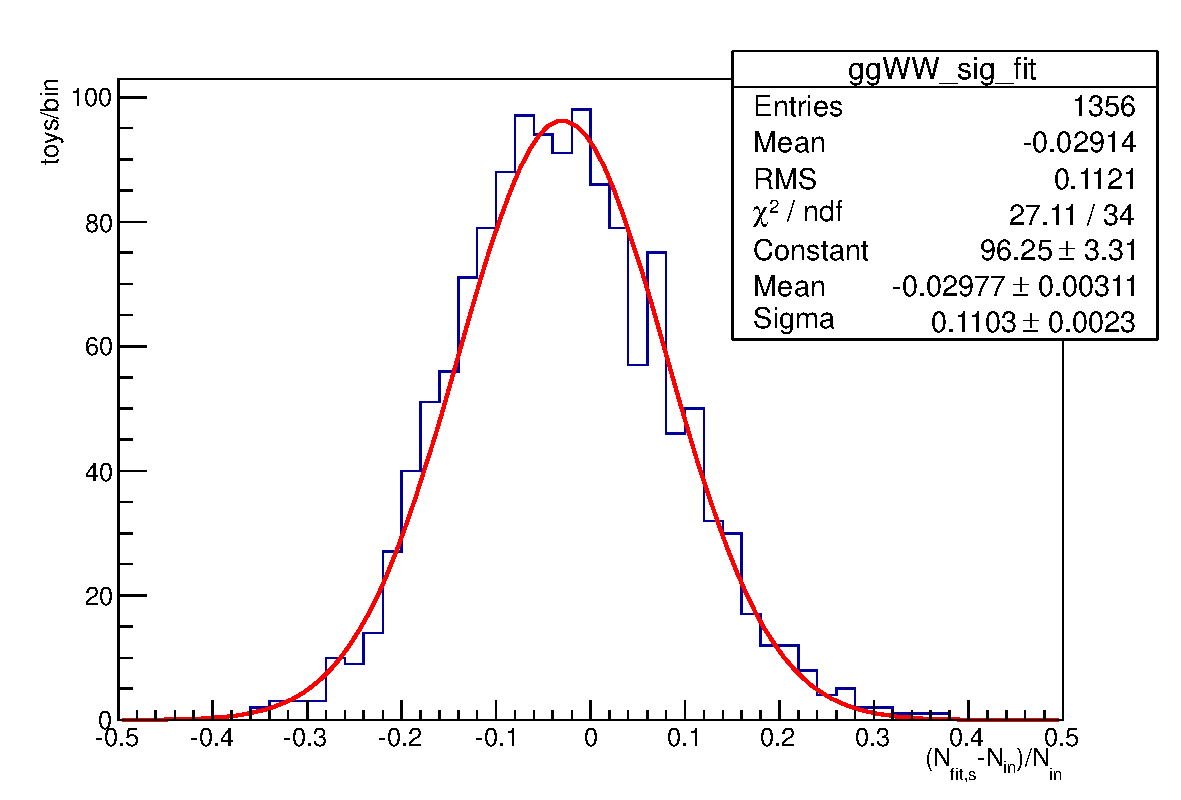
\includegraphics[width=.45\textwidth]{figures/norm_inj125_1j_125_sfit_ggWW_hww.pdf}
} 
\subfigure[Top]{
\centering
\label{subfig:top}
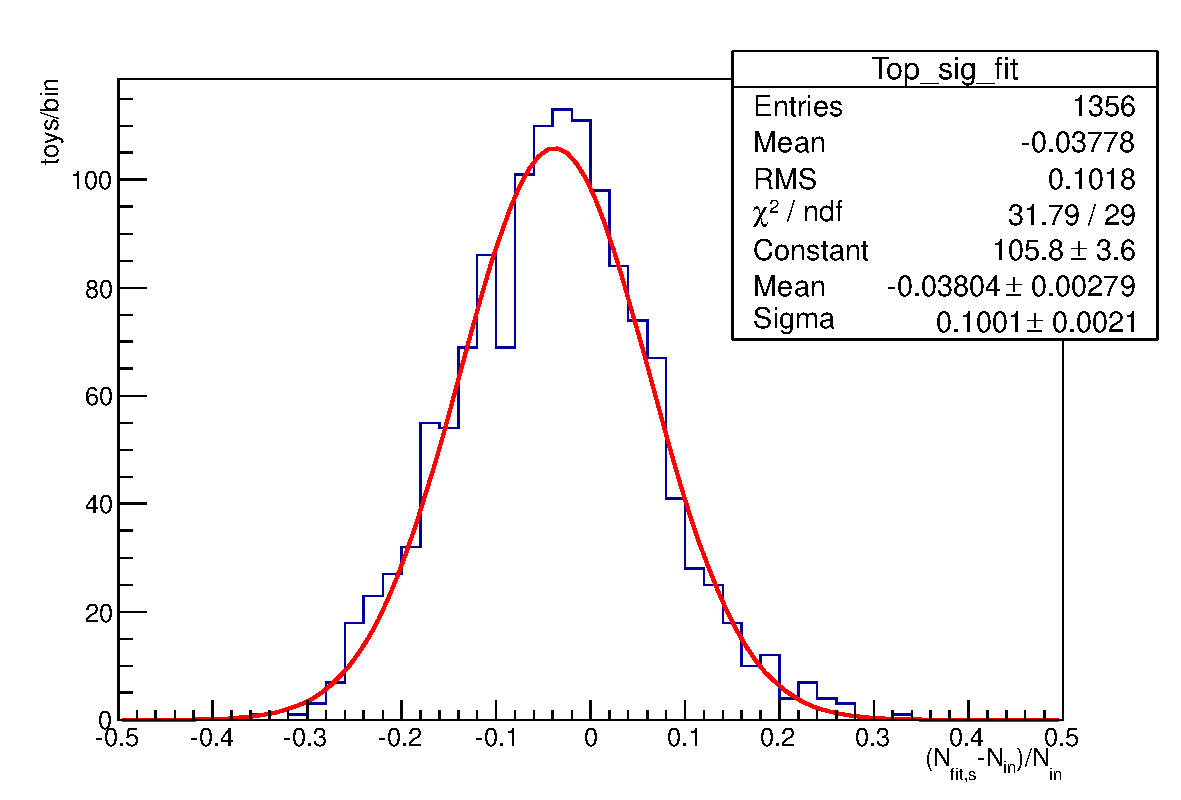
\includegraphics[width=.45\textwidth]{figures/norm_inj125_1j_125_sfit_Top_hww.pdf}
} \\
\subfigure[WjetsE]{
\centering
\label{subfig:wjetse}
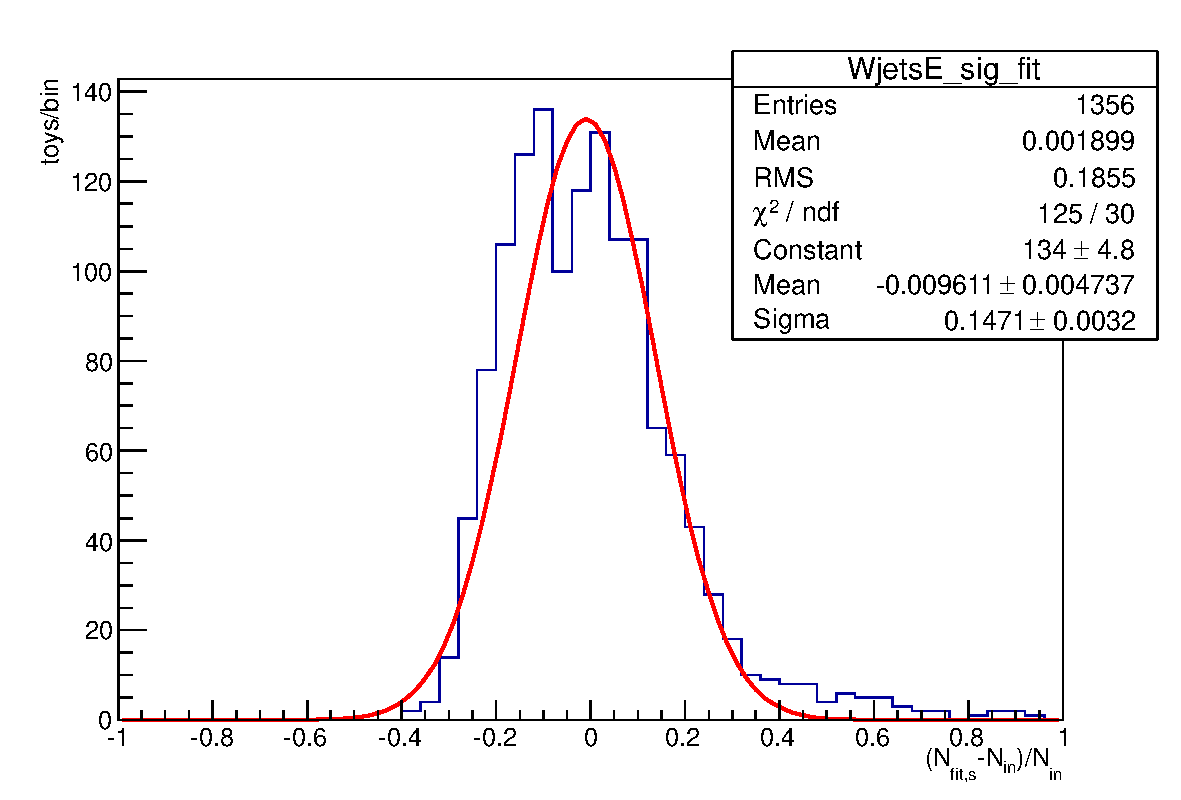
\includegraphics[width=.45\textwidth]{figures/norm_inj125_1j_125_sfit_WjetsE_hww.pdf}
} 
\subfigure[WjetsM]{
\centering
\label{subfig:wjetsm}
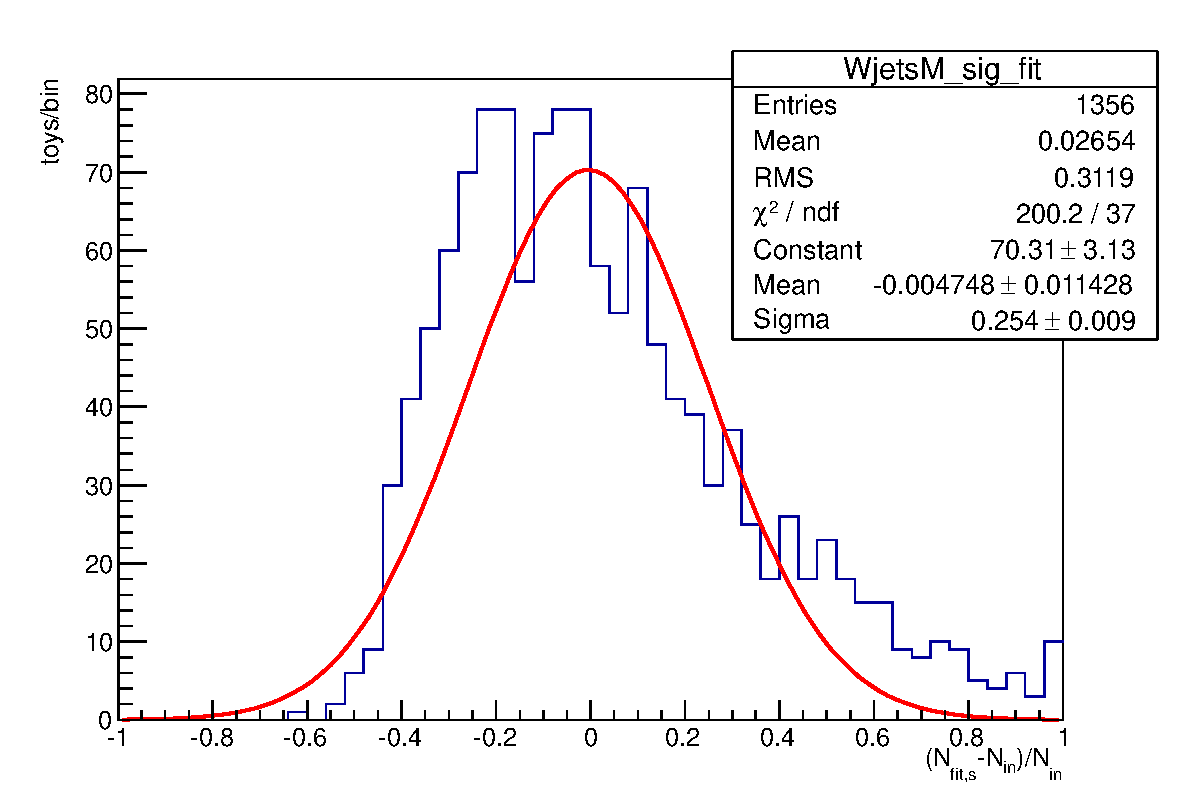
\includegraphics[width=.45\textwidth]{figures/norm_inj125_1j_125_sfit_WjetsM_hww.pdf}
} 
\subfigure[W$\gamma$]{
\centering
\label{subfig:wgamma}
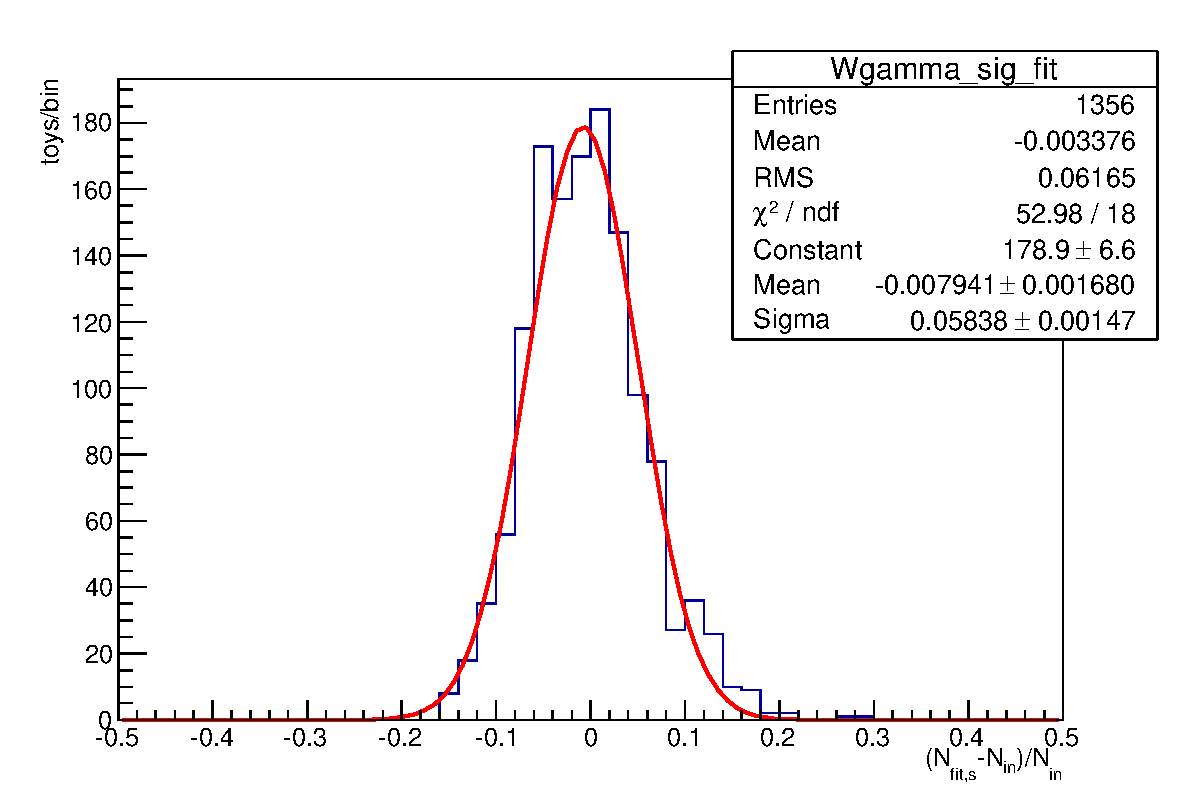
\includegraphics[width=.45\textwidth]{figures/norm_inj125_1j_125_sfit_Wgamma_hww.pdf}
} 
\subfigure[W$\gamma^*$]{
\centering
\label{subfig:wg3l}
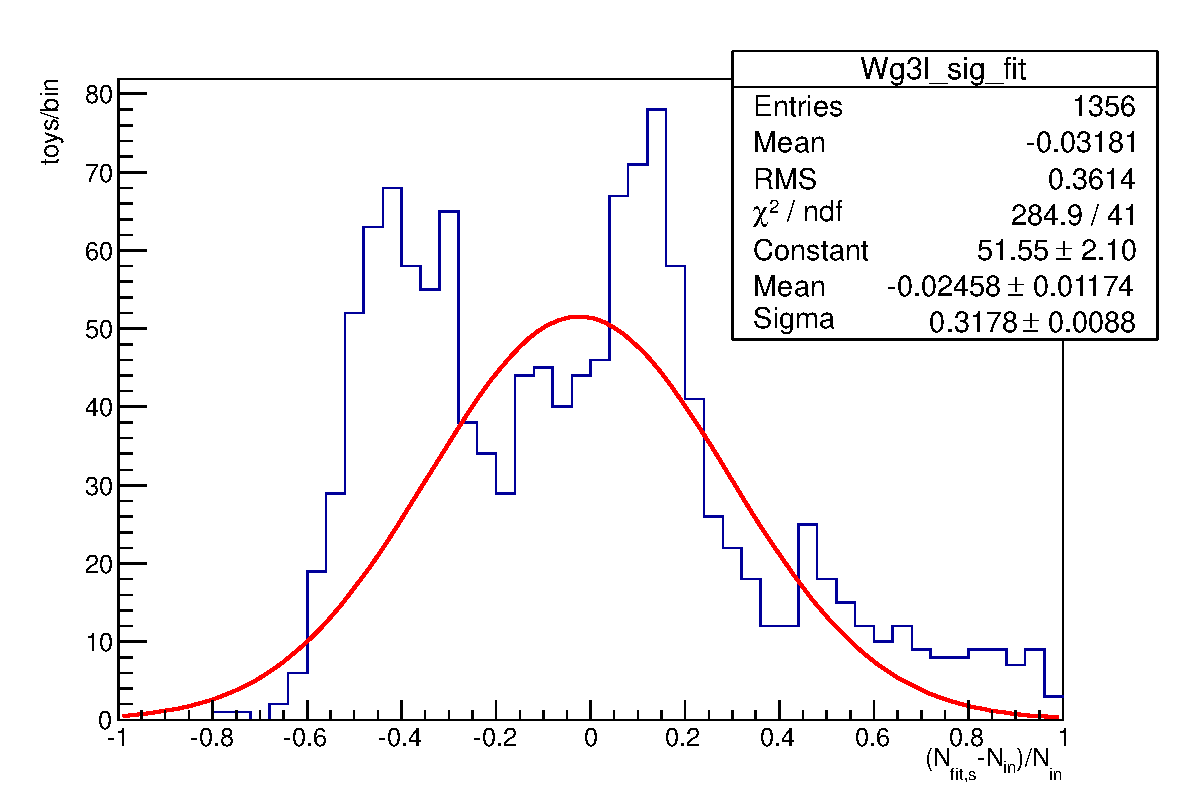
\includegraphics[width=.45\textwidth]{figures/norm_inj125_1j_125_sfit_Wg3l_hww.pdf}
} 

\caption{The relative fit bias $(N_{\text fit} - N_{\text in})/N_{\text in}$ distributions 
of the main signal and background processes in the toy MC based fit studies in the {\bf 1-Jet bin}. 
The toy datasets are generated sampling {\bf both statistics of the templates and systematic nusiances}. }
\label{fig:toyfit_1j}
\end{figure}
%%%%%%%%%%%%%%%%%%%%%%%%%%%%%%%%%%%%




In addition we tested the fit performance in case of problems with the main backgrounds, with the results summarized 
in Table~\ref{tab:toy_summary}.
\begin{itemize}

\item {\bf WjetsM} is a background with about two times as the total signal yield (Table~\ref{tab:yield_summary}) and it has a large normalization uncertainty (36\%). 
Its shape is well constrained but not very different from the signal one. 
Therefore, it is crucial to verify that the fit is stable with respect to WjetsM variations.
First, we tested the ability of the fit to distinguish the signal and WjetsM shapes by relaxing the WjetsM normalization 
without any input bias to the toys: the signal resolution is slightly degraded but no bias is introduced. 
Then, we applied an input bias ($\pm$1$\sigma$ normalization and shape) to the toys and analyzed them with the nominal analysis. 
The normalization bias is a large effect and the fit is only partially able to absorb it into the WjetsM component; 
the resulting bias on the signal is about 6\% (resolution is unaffected). 
The largest bias on the signal yield is 14\%, from the 1-Jet where the WjetsM background input is -36\% less than what 
the nominal fit assume.

\item {\bf qqWW} is the largest background; it is well constrained both in terms of normalization and shape, but small variations of this 
process have a large size with respect to the signal. 
We tested variations on normalization ($\pm$10\%, roughly equal to 1$\sigma$ in the 0-jet bin), 
on shape (using the alernative shape from MCatNLO as input to the toys) and on both. 
In all cases, the effect on the signal is small, with biases $\leq$1\% in the 0-Jet.  
%As expected, when relaxing the qqWW normalization uncertainty, it is easier for the fit to account the observed bias to the qqWW process,
%and consequently reduce the already small signal bias (by a factor of 2).

\item {\bf Top} is the main background in the 1-jet bin. 
We tested variations on normalization - $\pm$20\% (5\%), roughly equal to 1$\sigma$ in the 0-jet (1-jet) bin - and on shape 
(using the alernative shape from MadGraph as input to the toys) separately. No bias is introduced for the signal. 
It is interesting to note that, in case of normalization bias in the 1-jet bin, the fit prefers to account the observed bias 
into the qqWW component since it has similar shape but larger normalization error. However even in that case the impact 
on the signal yield is low being 6\%. 
\end{itemize}

In summary, we find the fit to be very stable with respect to biases at the level of 1$\sigma$ both in terms of shape and 
normalization for the main backgrounds. The largest observed bias is 14\% when injecting a 36\% less Wjets than expected 
in the 1-jet bin.
We also repeated the studies on the HCP analysis with results given in Appendix~\ref{sec:appendix_fittoyshcp}. 

%%%%%%%%%%%%%%%%%%%%%%%%%%%%%% 
\begin{table}
\begin{center}
\begin{tabular}{c | c  | c c | c c | c c | c c | c c }
\hline
          &      & \multicolumn{2}{c|}{{\bf ggH}} & \multicolumn{2}{c|}{qqWW} & \multicolumn{2}{c|}{Top} & \multicolumn{2}{c}{WjetsM} & \multicolumn{2}{c}{WjetsE} \\ 
N$_{jets}$ & Test & bias & $\sigma$ & bias & $\sigma$ & bias & $\sigma$ & bias & $\sigma$ & bias & $\sigma$ \\
\hline
0 & default                             &  2  & 28 & 0.4 & 3 & 0.4 & 11 & 0.5 & 15 & 0.7 & 10 \\
0 & sampling: stat.+syst.               & -3  & 35 & 0.6 & 6 &  2  & 19 &  4  & 23 &-0.6 & 11 \\
\hline
0 & analysis: inflated Wjets error      &  2  & 29 & -0.3 & 3 & 0.2 & 12 & -0.2      & 19 & -0.6 & 10 \\
0 & input: WjetsM {\bf +36\% bias}      &  6  & 28 & 0.3  & 3 & 0.8 & 11 & {\bf 27}  & 18 & 4    & 10 \\
0 & input: WjetsM {\bf -36\% bias}      & -6  & 25 & -1   & 3 & 3   & 11 & {\bf -23} & 10 & -7   & 10 \\
0 & input: WjetsM from altern. shape    & -4  & 25 & -0.1 & 3 & 2   & 11 & 6         & 15 & -0.5 & 10 \\
\hline
0 & input: qqWW {\bf +10\% bias}        & 0.7 & 28 & {\bf 10}  & 3 & 0.8 & 12 & 0.5 & 14 & 0.4 & 10 \\
0 & input: qqWW {\bf -10\% bias}        & 0.2 & 26 & {\bf -10} & 3 & 0.1 & 11 & 0.4 & 15 & 0.4 & 10 \\
0 & input: qqWW from altern. shape      & -2  & 27 & -0.1      & 3 & 2   & 12 & 6   & 15 & -2  & 10 \\
\hline
0 & input: Top {\bf +20\% bias}         & -2  & 27  & 1    & 3 & {\bf 11} & 12  & -0.5 & 15  & -1   & 9\\
0 & input: Top {\bf -20\% bias}         & 3   & 27  & -2   & 3 & {\bf -9} & 10  & 2    & 16  & -0.8 & 10\\
0 & input: Top from altern. shape       & -2  & 27  & -0.6 & 3 & 5        & 11  & 8    & 16  & -1   & 9\\
\hline
\hline
1 & default                             & -3  & 35 & 2   & 9  & -2  & 5 & -0.1 & 20 &-2 & 12 \\
1 & sampling: stat.+syst.               & -6  & 46 & 2   & 11 &-0.4 & 10& 0.5  & 25 & 1 & 15 \\
\hline
1 & analysis: inflated Wjets error      &  -3 &  37 & 2  & 9 & -2   & 5  & 0.1      & 24  & -2  & 12 \\ 
1 & input: WjetsM {\bf +36\% bias}      &  5  &  35 & 4  & 9 & -2   & 5  & {\bf 26} & 26  & 1   & 12 \\ 
1 & input: WjetsM {\bf -36\% bias}      & -14 &  33 & 0.5& 9 & -1   & 5  & {\bf-20} & 15  & -5  & 11 \\ 
1 & input: WjetsM from altern. shape    &  -3 &  35 & 1  & 8 & -0.3 & 5  & 17       & 21  & -1  & 12 \\
\hline
1 & input: qqWW {\bf +10\% bias}        & 4   & 37 & {\bf 12} & 9 & -2  & 5  & 0.3  & 19 & 1  & 11 \\
1 & input: qqWW {\bf -10\% bias}        & -1  & 33 & {\bf -7} & 9 & -2  & 5  & 0.3  & 18 & -2 & 13 \\
1 & input: qqWW from altern. shape      & -2  & 37 & 2        & 8 & -1  & 4  & 14   & 22 & -3 & 12 \\
\hline
1 & input: Top {\bf +5\% bias}          & -6   & 35  & 8   & 9 & {\bf -0.5} & 5 & -1 & 17 & -2 & 11 \\
1 & input: Top {\bf -5\% bias}          & -2   & 35  & -2  & 9 & {\bf -3}   & 5 & 2  & 19 & -1 & 12 \\
1 & input: Top from altern. shape       & -0.3 & 33  & 0.6 & 8 & 0.3        & 5 & 17 & 21 & -2 & 12 \\
\hline
\hline
\end{tabular}
\caption{Summary of results from toy experiments. Values of bias and $\sigma$ are \%.
In the Test column, ``default'' stands for: sampling is statistical only, input is nominal, analysis is nominal; 
in all other cases, the difference with respect to default is stated.}
\label{tab:toy_summary}
\end{center}
\end{table}


%%%%%%%%%%%%%%%%%%%%%%%%%%%%%% 
\begin{table}
\begin{center}
\begin{tabular}{c | c c c c c | c  c  c c c }
\hline
N$_{jets}$ & ggH & qqWW & Top & WjetsM & WjetsE & ggH/qqWW & ggH/Top & ggH/WjetsM & ggH/WjetsE \\
\hline
0 & 237.4 & 3930.1 & 488.9  & 512.4 & 276.4 & 6\% & 49\% & 46\% &  86\%\\
1 & 91.2  & 1177.5 & 1429.4 & 226.9 & 128.0 & 8\% & 64\% & 40\% &  71\%\\
\hline
\end{tabular}
\caption{Summary of yields and relative fraction of the signal with respect to the main backgrounds.}
\label{tab:yield_summary}
\end{center}
\end{table}

\subsection{Nuisance Parameters}

In this subsection we summarize the fit validation studies related to nuisance parameters.

The CL$_S$-LHC statistical method, used by all LHC Higgs analyses, prescribes that nuisance parameters are profiled in the fit, 
so that both their central value and the associated uncertainty can be varied. %fixme add reference
It is therefore important to establish which nuisance parameters the fit has to power to constrain, and then verify that the fit 
on data behaves as expected.

The model for the study of nuisances with toy experiments is sketched in Figure~\ref{fig:nuismodel}.
The nuisance model in the data card is here represented by the blue gaussian (the actual model is usually a log-normal distribution).
The central input value for this nuisance in the card correspond to $<$$nuis_{in}$$>$. 
Toys are thrown sampling the nuisance parameters according to their pdf; according to the assumed integrated luminosity, 
toys will also include variations of statistical nature. 
Therefore, the width of the nuisance model is $\sigma_{nuis,in} \oplus \sigma_{stat}$, and, when statistical effects are negligible, 
the width reduces to $\sigma_{nuis,in}$. 
For each toy experiment, the fit will determine a value $nuis_{fit}$ for the nuisance together with its post-fit uncertainty $\sigma_{nuis,fit}$.
In case the fit is able to constrain the parameter, $\sigma_{nuis,fit}$ will be smaller than $\sigma_{nuis,in}$; in case the fit is able to
determine the proper value for the nuisance parameter, the pull ($nuis_{fit}$-$<$$nuis_{in}$$>$)/$\sigma_{nuis,in}$ will have mean=0 and width $\sigma_w$=1.

%%%%%%%%%%%%%%%%%%%%%%%%%%%%%% 
\begin{figure}[!hbtp]
\centering
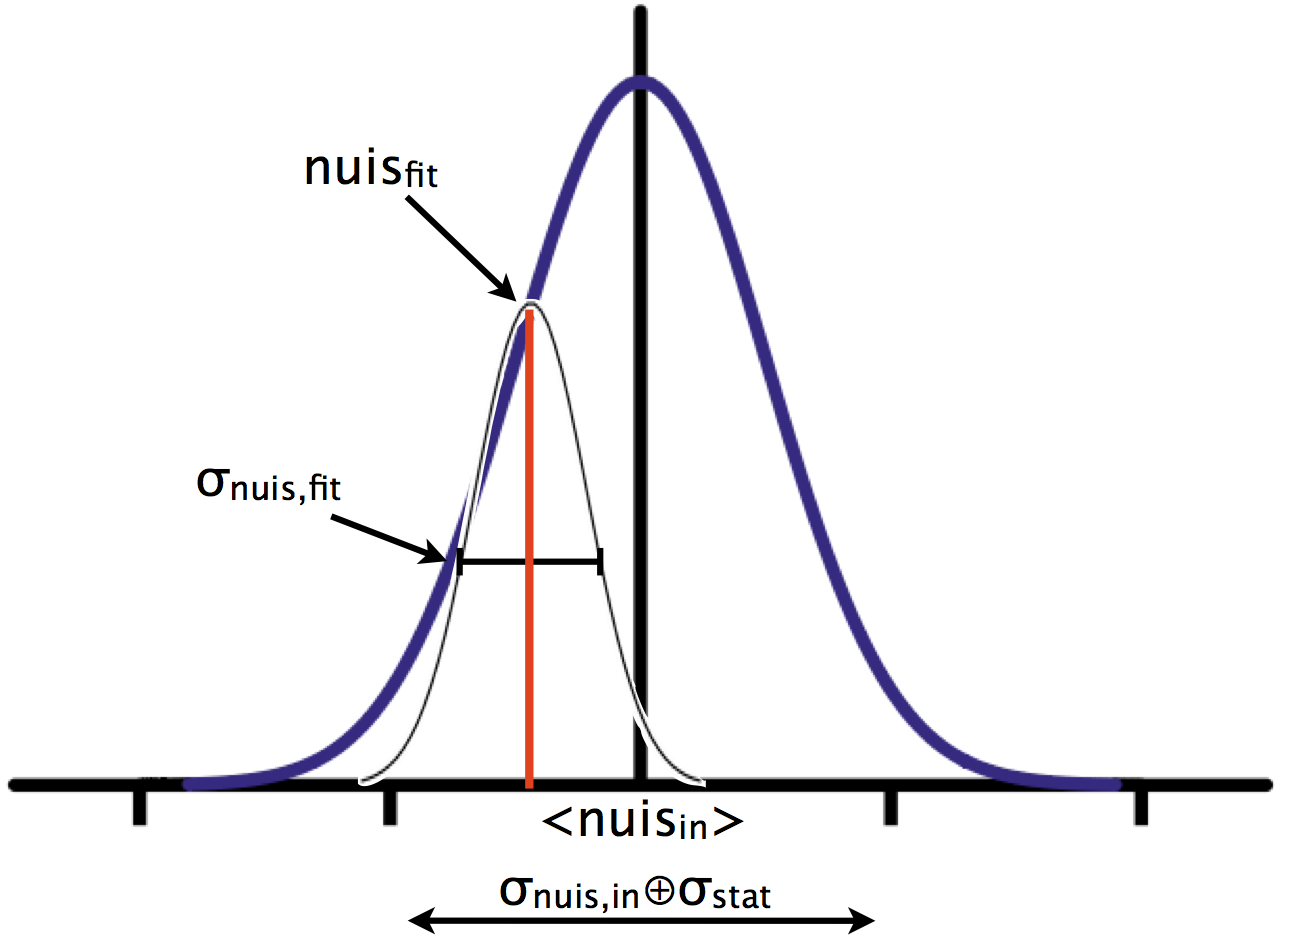
\includegraphics[width=.45\textwidth]{figures/nuismodel.png}
\caption{Model for the study of nuisance parameters with toy experiments.}
\label{fig:nuismodel}
\end{figure}
%%%%%%%%%%%%%%%%%%%%%%%%%%%%%% 

We initially test the fit behavior on a few simplified experiments. 
In this way, we learn how the fit deals with specific issues that will be also present in the full analysis fit.

\subsubsection{Results with Simplified Models}

First we test the fit using a very simple cut based data card (simplified model named v0), 
including only one signal process (ggH), one background process (qqWW) and one log-normal nuisance parameter (CMS\_hww\_0j\_WW\_8TeV)
corresponding to a 10\% background normalization uncertainty  (Table~\ref{tab:modelcutbased}).
Pseudo-data are generated according to this data card; each toy is then fit using the same card, where the data 
yield (and shape for shape-based analyses) is replaced with values from toy.

As shown in Figure~\ref{fig:sm_cut}, in this case, the fit is not able to constrain the nuisance parameter: 
the post-fit value and its uncertainty are identical to the input. 
This is expected because in the fit the signal strength is a free parameter and therefore the 
fit prefers to account all variations to signal rather than moving the nuisance parameter (a penalty has to be paid according to the nuisance model). 
The post-fit uncertainty on the signal strenght is about 38\%, as expected from the sum in quadrature of the statistical 
uncertainties on signal and background and the 10\% systematic uncertainty on the background.
The pull for the signal strenght parameter is unbiased with $\sigma_{w}$$\approx$1. 
Note that, unlike nuisance parameters, the pre-fit uncertainty is not defined for the signal strength parameter; 
therefore, its uncertainty is expressed as an absolute value (i.e. not normalized to input) and the post-fit uncertainty is used as denominator in the pull. 

%%%%%%%%%%%%%%%%%%%%%%%%%%%%%% 
\begin{table}[!hbtp]
\begin{center}
\begin{tabular}{l r c c}
\hline
process                &     & ggH & qqWW \\
rate                   &     & 88.9 & 294.8 \\
CMS\_hww\_0j\_WW\_8TeV & lnN &  -   & 1.100 \\
\hline
\end{tabular}
\caption{Simplified model for cut-based analysis v0.}
\label{tab:modelcutbased}
\end{center}
\end{table}
%%%%%%%%%%%%%%%%%%%%%%%%%%%%%% 


%%%%%%%%%%%%%%%%%%%%%%%%%%%%%%%%%%%%
\begin{figure}[!hbtp]
\centering
\subfigure[]{
\centering
\label{subfig:sm_cut_CMS_hww_0j_WW_8TeV_uncert}
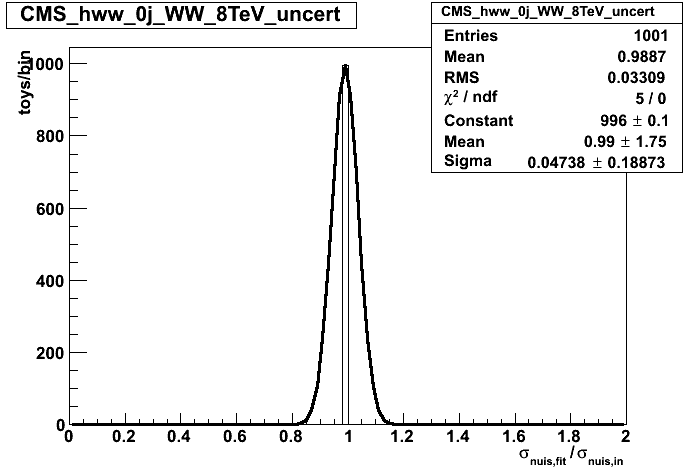
\includegraphics[width=.45\textwidth]{figures/sm_cut_CMS_hww_0j_WW_8TeV_uncert.png}
}
\subfigure[]{
\centering
\label{subfig:sm_cut_CMS_hww_0j_WW_8TeV_central}
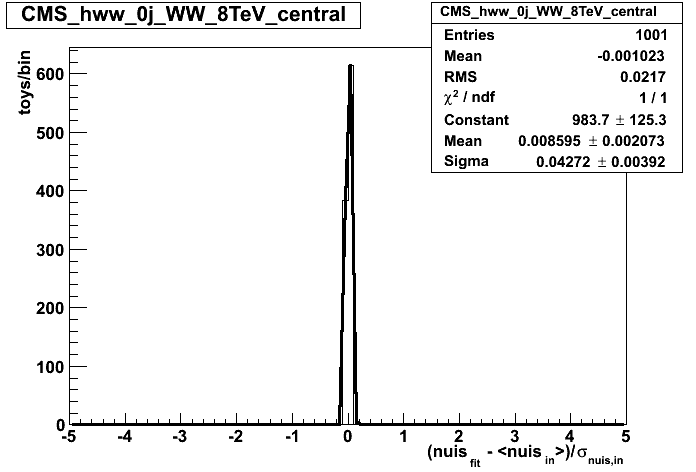
\includegraphics[width=.45\textwidth]{figures/sm_cut_CMS_hww_0j_WW_8TeV_central.png}
}\\
\subfigure[]{
\centering
\label{subfig:sm_cut_r_0j_uncert}
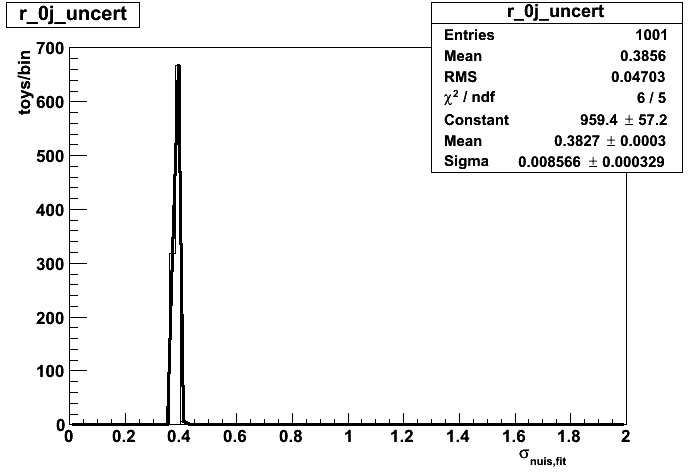
\includegraphics[width=.45\textwidth]{figures/sm_cut_r_0j_uncert.png}
}
\subfigure[]{
\centering
\label{subfig:sm_cut_r_0j_pull}
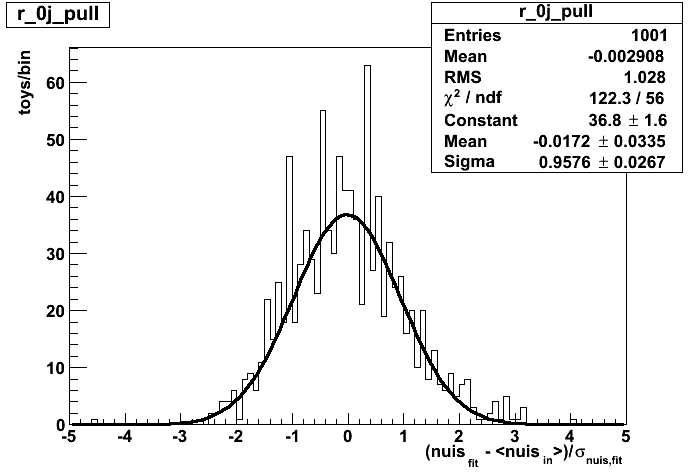
\includegraphics[width=.45\textwidth]{figures/sm_cut_r_0j_pull.png}
}
\caption{Results for cut based simplified model v0. Left column shows uncertainties, right column shows pulls.
First row is the qqWW normalization nuisance, second row is the signal strength.}
\label{fig:sm_cut}
\end{figure}
%%%%%%%%%%%%%%%%%%%%%%%%%%%%%%%%%%%%

The second simplified model is a shape analysis (v1). 
Again, it includes two processes only and, in addition to the 10\% normalization uncertainty, we also consider a shape 
uncertainty on the background (Table~\ref{tab:modelshapebased})\footnote{Note that CMS\_hww\_0j\_WW\_8TeV\_SHAPE is not
 a shape uncertainty but it is a normalization one used in the shape analysis. In this simple test it is log-normal (lnN), 
while in the full analysis it is flat (lnU).}.

In the shape analysis, the fit has a large control region to determine the qqWW normalization and shape; 
threfore, both the normalization and shape nuisances are constrained by the fit, with the uncertainty reduced 
by 80\% and 90\% respectively. The signal strength parameter has post-fit ucertainty $\sim$20\%.
On average no bias is observed and pulls have $\sigma_{w}$$\approx$1 (see Figure~\ref{fig:sm_shapev1}).

%%%%%%%%%%%%%%%%%%%%%%%%%%%%%% 
\begin{table}[!hbtp]
\begin{center}
\begin{tabular}{l r c c}
\hline
process                                   &       & ggH   & qqWW   \\
rate                                      &       & 228.1 & 3981.7 \\
CMS\_hww\_0j\_WW\_8TeV\_SHAPE             & lnN   &  -    & 1.100  \\
CMS\_hww\_MVAWWBounding                   & shape &  -    & 1.000  \\
\hline
\hline
CMS\_hwwof\_0j\_MVAqqWWStatBounding\_8TeV & shape &  -    & 1.000  \\
\hline
\end{tabular}
\caption{Simplified model for shape-based analyses. The upper block corresponds to v1, while v2 adds also the last line.}
\label{tab:modelshapebased}
\end{center}
\end{table}
%%%%%%%%%%%%%%%%%%%%%%%%%%%%%% 

%%%%%%%%%%%%%%%%%%%%%%%%%%%%%%%%%%%%
\begin{figure}[!hbtp]
\centering
\subfigure[]{
\centering
\label{subfig:sm_shapev1_CMS_hww_0j_WW_8TeV_SHAPE_uncert}
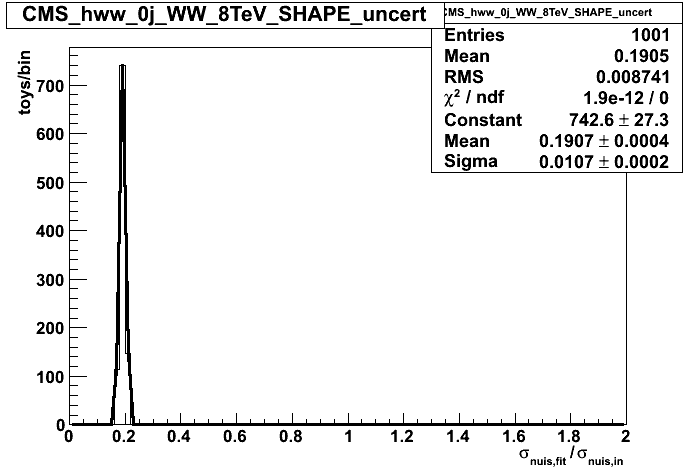
\includegraphics[width=.45\textwidth]{figures/sm_shapev1_CMS_hww_0j_WW_8TeV_SHAPE_uncert.png}
}
\subfigure[]{
\centering
\label{subfig:sm_shapev1_CMS_hww_0j_WW_8TeV_SHAPE_central}
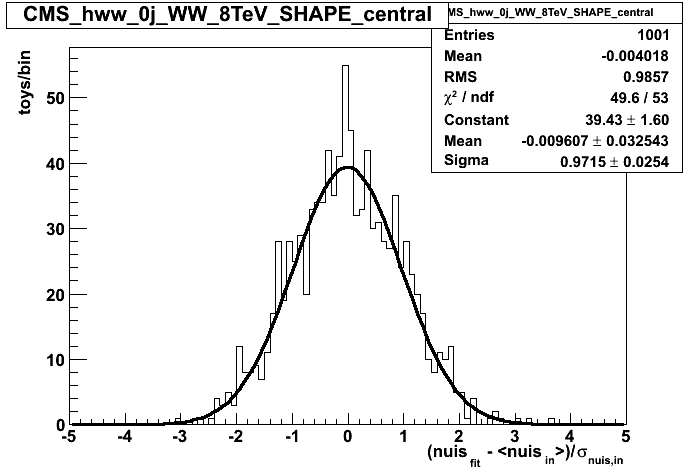
\includegraphics[width=.45\textwidth]{figures/sm_shapev1_CMS_hww_0j_WW_8TeV_SHAPE_central.png}
}\\
\subfigure[]{
\centering
\label{subfig:sm_shapev1_CMS_hww_MVAWWBounding_0j_uncert}
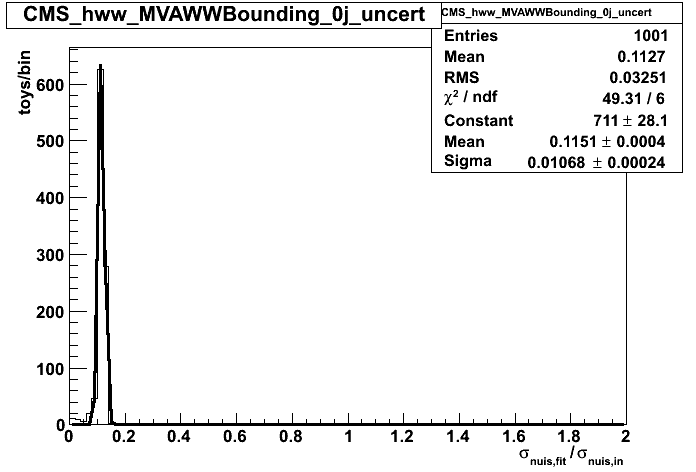
\includegraphics[width=.45\textwidth]{figures/sm_shapev1_CMS_hww_MVAWWBounding_0j_uncert.png}
}
\subfigure[]{
\centering
\label{subfig:sm_shapev1_CMS_hww_0j_MVAWWBounding_0j_central}
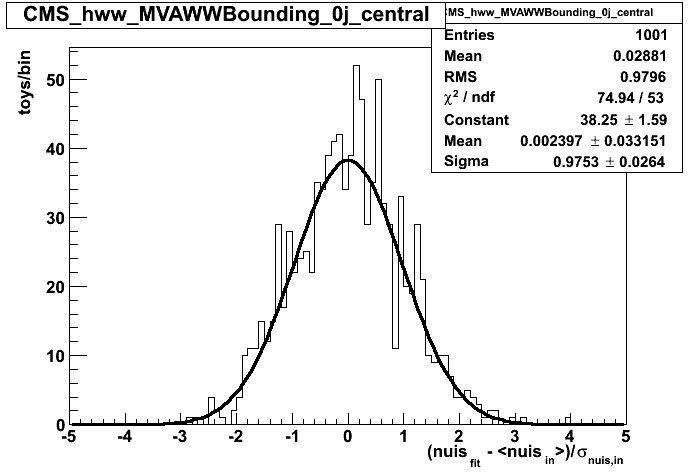
\includegraphics[width=.45\textwidth]{figures/sm_shapev1_CMS_hww_MVAWWBounding_0j_central.png}
}\\
\subfigure[]{
\centering
\label{subfig:sm_shapev1_r_0j_uncert}
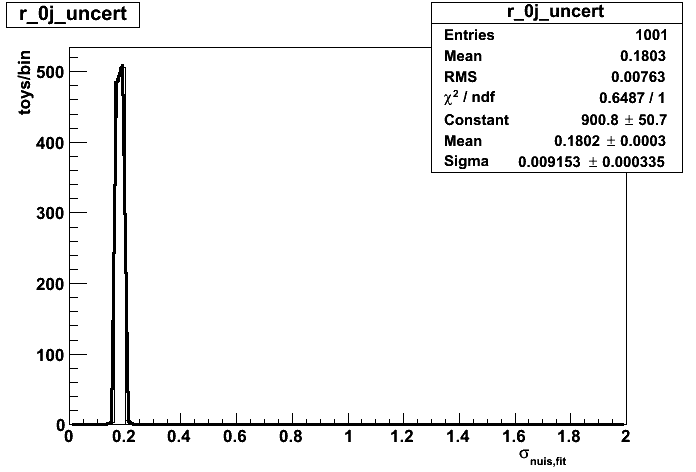
\includegraphics[width=.45\textwidth]{figures/sm_shapev1_r_0j_uncert.png}
}
\subfigure[]{
\centering
\label{subfig:sm_shapev1_r_0j_pull}
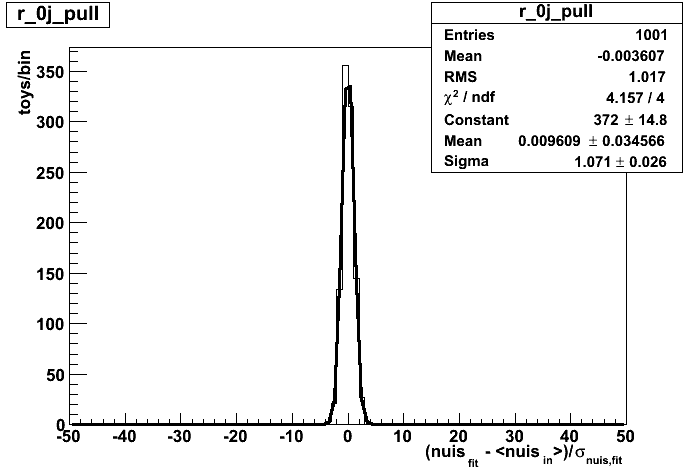
\includegraphics[width=.45\textwidth]{figures/sm_shapev1_r_0j_pull.png}
}
\caption{Results for shape-based simplified model v1. Left column shows uncertainties, right column shows pulls.
From top to bottom, rows correspond to the qqWW normalization nuisance, the qqWW shape nuisance and the signal strength.}
\label{fig:sm_shapev1}
\end{figure}
%%%%%%%%%%%%%%%%%%%%%%%%%%%%%%%%%%%%

We then modifiy the simplified model v1 by adding a second shape uncertainty (v2), corresponding to the statistical uncertainty for 
the background template (CMS\_hwwof\_0j\_MVAqqWWStatBounding\_8TeV). This additional unceratainty is strongly anti-correlated with the
normalization nuisance (correlation factor = -0.75), while it is not correlated to the other shape uncertainty.

The effect of the additional nuisance is that the fit has less power of determining the correlated nuisances: 
in fact (see Figure~\ref{fig:sm_shapev2}) the post-fit uncertainty for the normalization nuisance is larger than in v1 and the pulls of the
correlated nuisances have $\sigma_w$$<$1. 
The uncorrelated nuisance (CMS\_hww\_MVAWWBounding) and the signal strenght are barely affected, 
i.e. the signal is well measured even if some nuisances are not fully constrained.

%%%%%%%%%%%%%%%%%%%%%%%%%%%%%%%%%%%%
\begin{figure}[!hbtp]
\centering
\subfigure[]{
\centering
\label{subfig:sm_shapev2_CMS_hww_0j_WW_8TeV_SHAPE_uncert}
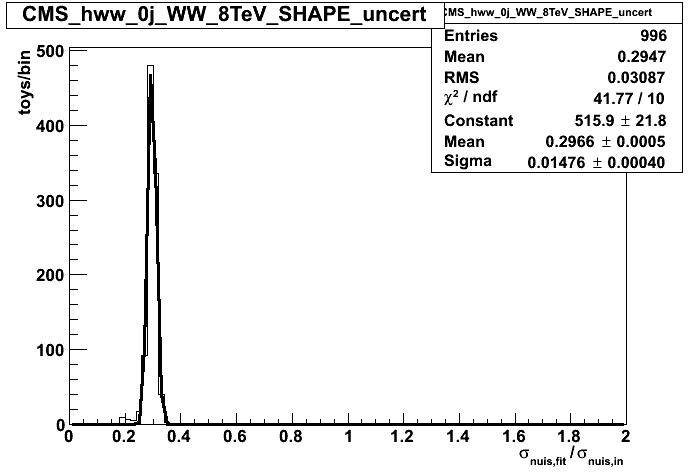
\includegraphics[width=.45\textwidth]{figures/sm_shapev2_CMS_hww_0j_WW_8TeV_SHAPE_uncert.png}
}
\subfigure[]{
\centering
\label{subfig:sm_shapev2_CMS_hww_0j_WW_8TeV_SHAPE_central}
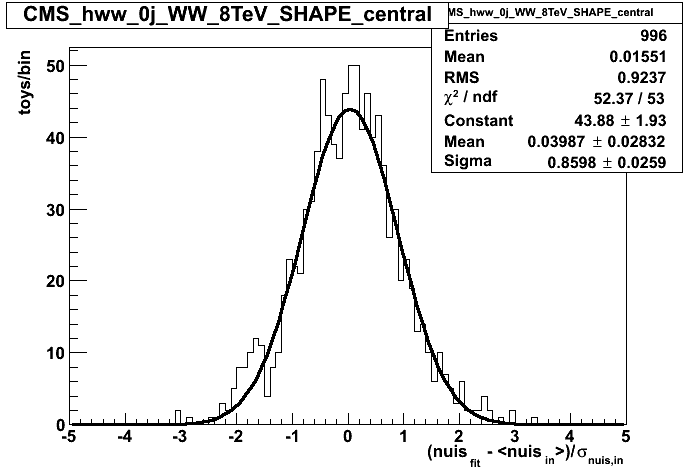
\includegraphics[width=.45\textwidth]{figures/sm_shapev2_CMS_hww_0j_WW_8TeV_SHAPE_central.png}
}\\
\subfigure[]{
\centering
\label{subfig:sm_shapev2_CMS_hww_MVAWWBounding_0j_uncert}
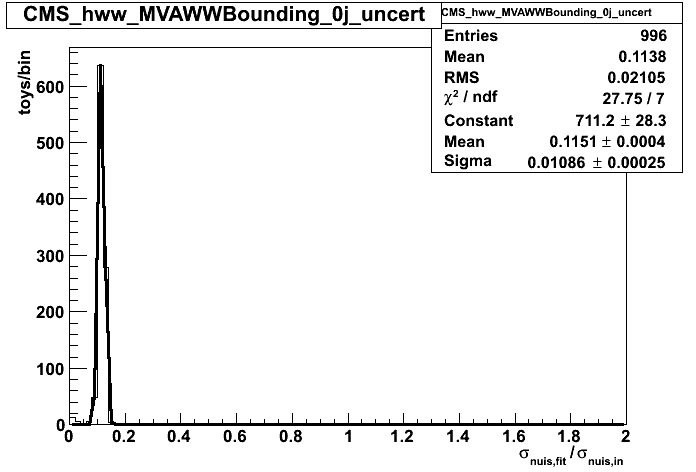
\includegraphics[width=.45\textwidth]{figures/sm_shapev2_CMS_hww_MVAWWBounding_0j_uncert.png}
}
\subfigure[]{
\centering
\label{subfig:sm_shapev2_CMS_hww_0j_MVAWWBounding_0j_central}
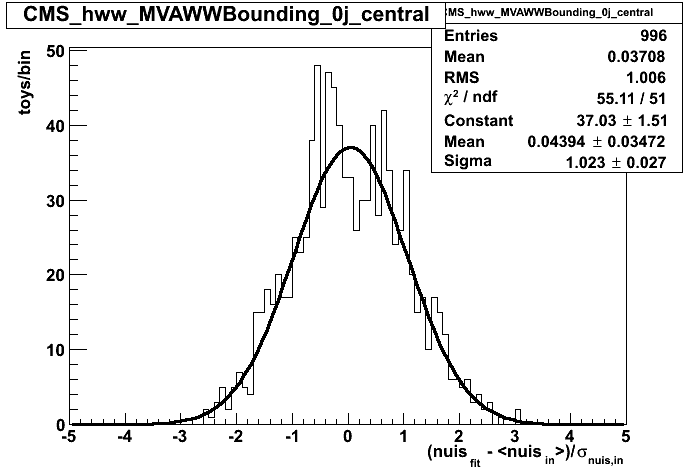
\includegraphics[width=.45\textwidth]{figures/sm_shapev2_CMS_hww_MVAWWBounding_0j_central.png}
}\\
\subfigure[]{
\centering
\label{subfig:sm_shapev2_CMS_hwwof_0j_MVAqqWWStatBounding_8TeV_uncert}
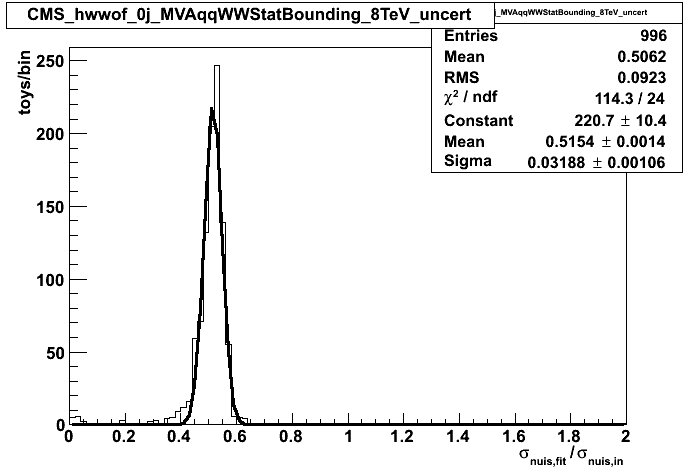
\includegraphics[width=.45\textwidth]{figures/sm_shapev2_CMS_hwwof_0j_MVAqqWWStatBounding_8TeV_uncert.png}
}
\subfigure[]{
\centering
\label{subfig:sm_shapev2_CMS_hwwof_0j_MVAqqWWStatBounding_8TeV_central}
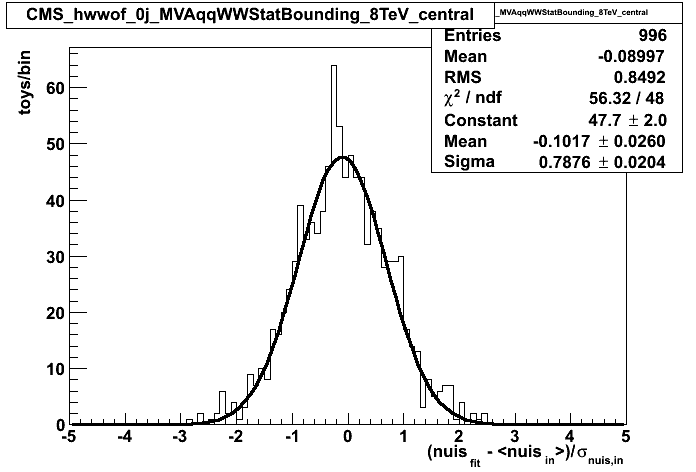
\includegraphics[width=.45\textwidth]{figures/sm_shapev2_CMS_hwwof_0j_MVAqqWWStatBounding_8TeV_central.png}
}\\
\subfigure[]{
\centering
\label{subfig:sm_shapev2_r_0j_uncert}
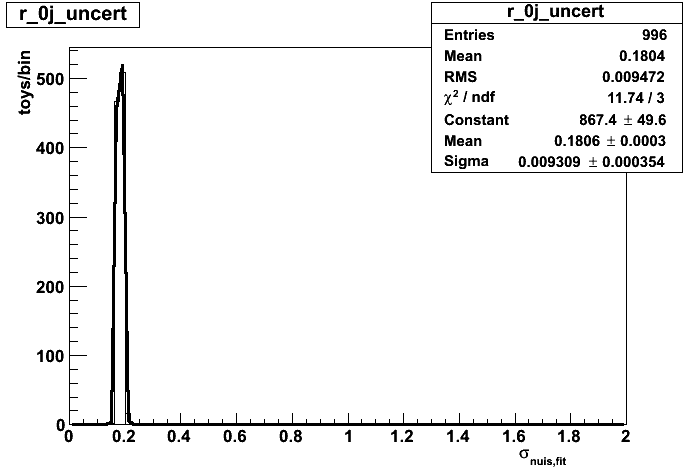
\includegraphics[width=.45\textwidth]{figures/sm_shapev2_r_0j_uncert.png}
}
\subfigure[]{
\centering
\label{subfig:sm_shapev2_r_0j_pull}
\includegraphics[width=.45\textwidth]{figures/sm_shapev2_r_0j_pull.png}
}
\caption{Results for shape-based simplified model v2. Left column shows uncertainties, right column shows pulls.
From top to bottom, rows correspond to the qqWW normalization nuisance, the qqWW shape nuisance, the qqWW template statistic nuisance 
and the signal strength.}
\label{fig:sm_shapev2}
\end{figure}
%%%%%%%%%%%%%%%%%%%%%%%%%%%%%%%%%%%%

In summary, simplified models teach us that:
\begin{itemize}
\item Cut based analysis is not able to constrain the nuisances which stick to input values; all variations are accounted by signal (free to float);
\item Shape based analysis does constrain the nuisances, both shape and normalization ones; 
in this case, uncertainties are reduced by 80-90\% and pulls have width $\sim$1;
\item When many correlated nuisances are present, the fit loses constraining power and pulls may have width$<$1;
\item Signal strength shows unbiassed pulls with width $\sim$1 both in cut and shape based analysis.
\end{itemize}

\clearpage

\subsubsection{HWW Analysis Results}

We now validate the post-fit values for the nuisance parameters in the HWW analysis.
In this test we consider the most sensitive channel, i.e. 0-jet, DF, 8TeV, 2D shape (correlations with other channels not taken into account).
Pseudo-data are generated according to the corresponding data card, with the only difference that the qqWW normalization systematic is assumed to be
log-normal with 10\% uncertainty (using flat uncertainty would lead to instability problems in the generation of toys).
Each toy is then fitted using the default card (i.e. flat qqWW normalization uncertainty), where the data yield and shape are replaced with those from the toy.

From the simplified models we expect that normalization nuisances not related to a specific shape are not constrained by fit, 
that nuisances related to the shape of dominant backgrounds are strongly constrained by the data fit and that, when many nuisances are correlated, 
the fit constraining power is reduced.

Results for all the $\sim$50 nuisance parameters in the data cards are impractical to present, 
so we have collected a few representative cases in Figure~\ref{fig:nuis2D0jdf8Tev}.
The nuisance related to luminosity (\ref{subfig:lumi_8TeV_0j_uncert} and \ref{subfig:lumi_8TeV_0j_central}) is a normalization uncertainties correlated 
among all processes taken from MC. 
In this case the fit is not able to determine the nuisance and sticks close to the input values; a similar picture is observed for several other nuisances: 
e.g. normalization or shape of minor backgrounds, many theoretical uncertainties.
Shape nuisances can also be poorly constrained: as an example, WjetsE (\ref{subfig:CMS_hww_MVAWEBounding_0j_uncert} and \ref{subfig:CMS_hww_MVAWEBounding_0j_central}) 
is a process that is difficult to separate from the signal (uncertainty reduced by $\sim$6\%, pull width $\sim$0.2).
On the contrary, the fit can constrain WW background in the high \mt\ and \mll\ regions; therefore, its shape uncertainty 
(\ref{subfig:CMS_hww_MVAWWBounding_0j_uncert} and \ref{subfig:CMS_hww_MVAWWBounding_0j_central}) is strongly constrained by the fit, 
having the uncertainty reduced to 17\% and a pull width not far from 1.
The shape uncertainty related to the MET resolution (\ref{subfig:CMS_hww_MVAMETResBounding_0j_uncert} and \ref{subfig:CMS_hww_MVAMETResBounding_0j_central}) is constrained
by the fit, with a 50\% uncertainty reduction and a pull width $\sim$0.8.
Finally, the signal strenght, shows an average post-fit uncertainty of $\sim$25\% and a pull with mean $\sim$0.2 and width $\sim$1.0.
The magenta line in the plots corresponds to the result of the real data fit: in all cases it is reasonably compatible with the expectation from toys.

%%%%%%%%%%%%%%%%%%%%%%%%%%%%%%%%%%%%
\begin{figure}[!hbtp]
\centering
\subfigure[]{
\centering
\label{subfig:lumi_8TeV_0j_uncert}
\includegraphics[width=.35\textwidth]{figures/lumi_8TeV_0j_uncert.png}
}
\subfigure[]{
\centering
\label{subfig:lumi_8TeV_0j_central}
\includegraphics[width=.35\textwidth]{figures/lumi_8TeV_0j_central.png}
}\\
\subfigure[]{
\centering
\label{subfig:CMS_hww_MVAWWBounding_0j_uncert}
\includegraphics[width=.35\textwidth]{figures/CMS_hww_MVAWWBounding_0j_uncert.png}
}
\subfigure[]{
\centering
\label{subfig:CMS_hww_MVAWWBounding_0j_central}
\includegraphics[width=.35\textwidth]{figures/CMS_hww_MVAWWBounding_0j_central.png}
}\\
\subfigure[]{
\centering
\label{subfig:CMS_hww_MVAWEBounding_0j_uncert}
\includegraphics[width=.35\textwidth]{figures/CMS_hww_MVAWEBounding_0j_uncert.png}
}
\subfigure[]{
\centering
\label{subfig:CMS_hww_MVAWEBounding_0j_central}
\includegraphics[width=.35\textwidth]{figures/CMS_hww_MVAWEBounding_0j_central.png}
}\\
\subfigure[]{
\centering
\label{subfig:CMS_hww_MVAMETResBounding_0j_uncert}
\includegraphics[width=.35\textwidth]{figures/CMS_hww_MVAMETResBounding_0j_uncert.png}
}
\subfigure[]{
\centering
\label{subfig:CMS_hww_MVAMETResBounding_0j_central}
\includegraphics[width=.35\textwidth]{figures/CMS_hww_MVAMETResBounding_0j_central.png}
}\\
\subfigure[]{
\centering
\label{subfig:r_0j_uncert}
\includegraphics[width=.35\textwidth]{figures/r_0j_uncert.png}
}
\subfigure[]{
\centering
\label{subfig:r_0j_pull}
\includegraphics[width=.35\textwidth]{figures/r_0j_pull.png}
}
\caption{Highlights of results for 0-jet, DF, 8TeV, 2D shape analysis. The vertical line in magenta corresponds to the real data result.
Left column shows uncertainties, right column shows pulls. From top to bottom, rows correspond to luminosity nuisance, qqWW shape nuisance, 
WjetsE shape nuisance, MET resolution shape nuisance and signal strength.}
\label{fig:nuis2D0jdf8Tev}
\end{figure}
%%%%%%%%%%%%%%%%%%%%%%%%%%%%%%%%%%%%

The nuisance parameters whose uncertainty is reduced by $>$30\% after the fit are WW shapes ($\sim$85\% reduction), Top shape ($\sim$70\% reduction), 
lepton and MET resolutions ($\sim$50\% reduction).
The first two are expected because the analysis is designed precisely to determine WW (primarily) and Top (secondarily) in signal-free regions, 
where the large input variations can be constrained by the fit.
On the other hand, the fact that the fit constrains some nuisances related to experimental effects may be a bit surprising and is not expected.
One could argue that the fit is able to measure lepton and MET resolutions with a better precision than what was provided as input.
However, such resolutions are not “directly” fitted (e.g. from the width of the Z peak) but they convolute with other effects resulting in 
the \mt-\mll\ shape for each process; therefore, we do not think the present fit provides a reliable measurement of such quantities.
In any case, variations due to these effects in the signal region are very small and will not affect the main analysis result.
In fact, we have verified that assuming different models for such nuisances (i.e. removing the experimental effect nuisances or replacing 
the shape uncertainty with a corresponding normalization uncertainty), the final result is almost unchanged.

In summary, we observe that:
\begin{itemize}
\item All nuisance pulls are unbiased;
\item Many nuisances are not constrained at all by the fit (post-fit value and uncertainty almost identical to input): 
these are mainly theoretical uncertainties, luminosity, minor backgrounds;
\item Several nuisance parameters are constrained by the fit; in particular, the uncertainty on shape and normalization of main backgrounds is strongly reduced;
\item The signal strength has an average unceratinty of 35\% and its pull has mean $\sim$0.2 and width $\approx$1;
\item Data results are fully compatible with expectations from toys.
\end{itemize}
Therefore, we can conclude that the nuisance parameters are under control in the fit.
